\chapter*{Anhang}\label{Anhang}

\begin{tabular}{ll}
\bf Anhang \ref{Anhang_Glossar}: &\bf Glossar\\
\bf Anhang \ref{Anhang_Algorithmen}: &\bf Algorithmen\\
\bf Anhang \ref{Anhang_Beispiele}: &\bf Lösungsstrategien an Beispielen
\end{tabular}

\chapter{Glossar}\label{Anhang_Glossar}

\begin{tabular}{lp{12cm}cm{1cm}}
\textbf{Bezeichner} & \textbf{Bedeutung} & \textbf{Seite}\\
\hline
$a \in \mathbb{N}$ 
& \textbf{Feld} eines Gartens
& \pageref{Felder}\\

$G=(V,E)$
& \textbf{Graph}, durch den der Garten modellhaft beschrieben wird
& \pageref{Graph}\\

$V$
& \textbf{Knotenmenge} des Graphen $G$; entspricht den Feldern des durch $G$ modellierten Gartens
& \pageref{Knotenmenge}\\

$E$
& \textbf{Kantenmenge} des Graphen $G$; beschreibt die Nachbarschaft der Felder des durch $G$ modellierten Gartens
& \pageref{Kantenmenge}\\

$C$
& \textbf{Bewertungsmatrix} eines kantenbewerteten Graphen
& \pageref{Bewertungsmatrix}\\

$D$
& \textbf{Entfernungsmatrix} eines kantenbewerteten Graphen
& \pageref{Entfernungsmatrix}\\

$s: V \rightarrow V$ 
& \textbf{Nachfolgerfunktion}, wenn die \textit{Nachbarschaftsbedingung} (\ref{HJKmlp_equation_Nachbarschaftsbedingung}) gilt und der durch $s$ $\rightarrow$\textit{induzierte Teilgraph} $\vec{G}_s$ zyklenfrei ist
& \pageref{Nachfolgerfunktion}\\

$\vec{G}_s = \langle V,\vec{E}_s \rangle$
& durch die $\rightarrow$\textit{Nachfolgerfunktion} $s$ \textbf{induzierter Teilgraph} von $G=(V,E)$ mit $\vec{E}_s = \{\langle a,s(a)\rangle \mid a\in V \wedge a \neq s(a)\}$
& \pageref{induzierter Teilgraph}\\

$h \in V$
& \textbf{Haufenfeld} oder \textbf{Hub} $\equiv$ Senke des durch die $\rightarrow$\textit{Nachfolgerfunktion} $s$ $\rightarrow$\textit{induzierten Teilgraphen} $\vec{G}_s$, d.h. $s(h)=h$
& \pageref{Hub}\\

$Hub(s)$
& \textbf{Hubmenge} $\equiv$ Menge aller $\rightarrow$\textit{Haufenfelder} ($\rightarrow$\textit{Hubs}), welche durch die $\rightarrow$\textit{Nachfolgerfunktion} $s$ induziert werden 
& \pageref{Hubmenge}\\

$q \in V$
& \textbf{Harkquelle} $\equiv$ Quelle des durch die $\rightarrow$\textit{Nachfolgerfunktion} $s$ $\rightarrow$\textit{induzierten Teilgraphen} $\vec{G}_s$
& \pageref{Harkquelle}\\

$Q(s)$
& \textbf{Harkquellenmenge} $\equiv$ Menge aller $\rightarrow$\textit{Harkquellen}, welche durch die $\rightarrow$\textit{Nachfolgerfunktion} $s$ induziert werden 
& \pageref{Harkquellenmenge}\\

$K \in V$
& \textbf{Kompostfeld} $\equiv$ Kompoststelle des Gartens
& \pageref{Kompostfeld}\\

$M(a)$ 
& initiale \textbf{Laubmenge} in $\rightarrow$\textit{Feld} $a$; entspricht der Knotenbewertung des  $\rightarrow$\textit{Graphen} $G$
& \pageref{Laubmenge}\\

$M^*(a)$
& \textbf{aktuelle Laubmenge} in $\rightarrow$\textit{Feld} $a$; gibt die (zwischenzeitlich) kumulierte Laubmenge in Feld $a$ zum Zeitpunkt des Harkens von Feld $a$ zu einem Nachbarfeld an
& \pageref{aktuelle Laubmenge}\\

$M_k$
& \textbf{kritische Laubharkmenge}; entspricht der Laubmenge, die noch mit einem einzigen Harkzug bewegt werden kann
& \pageref{kritische Laubharkmenge}\\

$\overline{M}, \overline{M}(a)$
& \textbf{maximale Laubmenge} (von $\rightarrow$\textit{Feld} $a$); entspricht der Laubmenge, die maximal im Feld $a$ angehäuft werden kann
& \pageref{maximale Laubmenge}\\

$M^*_s:V \rightarrow \mathbb{R}_\geq$
& die durch die $\rightarrow$\textit{Nachfolgerfunktion} $s$ induzierte \textbf{Anhäufungsfunktion} gemäß Bildungsvorschrift (\ref{Definition_Anhäufungsfunktion})
& \pageref{Anhäufungsfunktion},\pageref{Anhäufungsfunktion_2} \\
\end{tabular}



\begin{tabular}{lp{11cm}cm{1cm}}
\textbf{Bezeichner} & \textbf{Bedeutung} & \textbf{Seite}\\
\hline

$\alpha_H$, $\alpha_H(a,b)$
& \textbf{Harkaufwandsfaktor} oder \textbf{Harkparameter}
& \pageref{Harkaufwandsfaktor}\\

$HA(a,b)$
& einzelner \textbf{Harkaufwand}; entspricht dem Aufwand für das Harken der aktuellen Laubmenge von Feld $a$ in ein benachbartes Feld $b$
& \pageref{Harkaufwand}f\\

$HA_{\Sigma}(s)$
&\textbf{Harkaufwandsumme}; entspricht dem Gesamtaufwand des produktiven Harkprozesses, der durch die $\rightarrow$\textit{Nachfolgerfunktion} $s$ beschrieben wird
&\pageref{Formel_Harkaufwandsumme}\\

$\alpha_W$, $\alpha_W(a,q)$
& \textbf{Wegeaufwandsfaktor} oder \textbf{Wegeparameter}
& \pageref{Wegeaufwandsfaktor}\\

$W(s)$
&\textbf{unproduktive Weglänge}; entspricht der Gesamtlänge aller unproduktiven Wege, welche durch die $\rightarrow$\textit{Nachfolgerfunktion} $s$ hervorgerufen werden
& \pageref{Wegeaufwandsfaktor}\\

$WA_{\Sigma}(s)$
&\textbf{unproduktiver Wegeaufwand}; entspricht dem Gesamtaufwand für unproduktive Wege des durch die $\rightarrow$\textit{Nachfolgerfunktion} $s$ beschriebenen Harkprozesses
& \pageref{Wegeaufwandsfaktor}f\\

$\alpha_T$
& \textbf{Transportaufwandsfaktor} oder \textbf{Transportparameter}
& \pageref{Transportaufwandsfaktor}\\

$\overline{T}$
& \textbf{maximales Ladevolumen} des Transportmittels
& \pageref{Ladevolumen}\\

$\gamma$
& \textbf{variabler Ladeaufwand} $\equiv$ variabler Aufwandsanteil für Auf- und Abladen einer Laubmenge 
& \pageref{variabler Ladeaufwand}\\

$\sigma$
& \textbf{fixer Ladeaufwand} $\equiv$ fixer Aufwandsanteil für Auf- und Abladen einer Laubmenge
& \pageref{fixer Ladeaufwand}\\

$TA(h)$
& \textbf{Transportaufwand} von $\rightarrow$\textit{Hub} $h$ zum $\rightarrow$\textit{Kompostfeld} $K$; entspricht dem Aufwand für das Transportieren der kumulierten Laubmenge von $\rightarrow$\textit{Hub} $h$ zum $\rightarrow$\textit{Kompostfeld} $K$, einschließlich der Aufwände für das Auf- und Abladen
& \pageref{Transportaufwandsfaktor}\\

$TA_{\Sigma}(s)$
& \textbf{Transportaufwandsumme}; ergibt sich als gesamter Transportaufwand aller Touren zwischen allen $\rightarrow$\textit{Hubs} bzgl. $\rightarrow$\textit{Nachfolgerfunktion} $s$ und $\rightarrow$\textit{Kompostfeld}, einschließlich aller Aufwände für das Auf- und Abladen
&\pageref{Transportaufwandsformel_5}\\

$M^{**}_s(h)$
&eine nach entsprechend vielen Pendeltouren verbleibende \textbf{Laubrestmenge} beim $\rightarrow$\textit{Hub} $h$
&\pageref{Laubrestmenge}\\

$\pi:V \leftrightarrow V$
& Permutation zur \textbf{Ausrichtung} einer $\rightarrow$\textit{Nachfolgerfunktion} $s$
& \pageref{Ausrichtung}\\

$R(a)$
&\textbf{Erreichbarkeitsmenge}; enthält alle Knoten $i \in V$, von denen aus der Knoten $a$ entlang einer Pfeilfolge im $\rightarrow$\textit{induzierten Teilgraph} $\vec{G}_s$ erreichbar ist
& \pageref{Erreichbarkeitsmenge},\pageref{Erreichbarkeitsmenge_2}\\

$C(h)$
& \textbf{Cluster}; entspricht der $\rightarrow$\textit{Erreichbarkeitsmenge} einer Senke $h$ des  $\rightarrow$\textit{induzierten Teilgraphen} $\vec{G}_s$
&\pageref{Cluster}\\

$\Lambda(G)$
& \textbf{Lösungsraum} des Laubharkproblems 
&\pageref{Lambda}\\

$K$
& \textbf{Kostenfunktion} als Zielfunktion des Laubharkproblems
&\pageref{Kostenfunktion}\\

\end{tabular}

































\chapter{Algorithmen}\label{Anhang_Algorithmen}

\begin{tabular}{lp{10cm}cm{2cm}}
\textbf{Lfd. Nr.} & \textbf{Bezeichnung} & \textbf{Seite}\\
\hline
Algorithmus \ref{Algo_Prüfung_Nachfolgerfunktion}: 
& Prüfung der Bedingungen einer Nachfolgerfunktion 
& \pageref{Algo_Prüfung_Nachfolgerfunktion}\\

Algorithmus \ref{Algo_Zulässigkeitsprüfung}: 
& Zulässigkeitsprüfung für Nachfolgerfunktion 
& \pageref{Algo_Zulässigkeitsprüfung}\\

Algorithmus \ref{Algo_Erreichbarkeitsmengenbestimmung}: 
& Bestimmung einer Erreichbarkeitsmenge 
& \pageref{Algo_Erreichbarkeitsmengenbestimmung}\\

Algorithmus \ref{Algo_Clusterbestimmung}: 
& Clusterbestimmung 
& \pageref{Algo_Clusterbestimmung}\\

Algorithmus \ref{Algo_Bestimmung_Harkaufwand}: 
& Berechnung des Harkaufwandes 
& \pageref{Algo_Bestimmung_Harkaufwand}\\

Algorithmus \ref{Algo_unproduktive_Wege}: 
& Berechnung des unproduktiven Wegeaufwandes 
& \pageref{Algo_unproduktive_Wege}\\

Algorithmus \ref{Algo_Ausrichtung_Nachfolgerfunktion}: 
& Ausrichtung einer Nachfolgerfunktion 
& \pageref{Algo_Ausrichtung_Nachfolgerfunktion}\\

Algorithmus \ref{Algo_Berechnung_von_HA_und_HW}: 
& Berechnung von Hark- und Wegeaufwand anhand einer ausgerichteten Nachfolgerfunktion 
& \pageref{Algo_Berechnung_von_HA_und_HW}\\

Algorithmus \ref{Algo_Berechnung_von_Transportaufwänden}: 
& Berechnung von Transportaufwänden 
& \pageref{Algo_Berechnung_von_Transportaufwänden}\\

Algorithmus \ref{Algo_Zickzack}: 
& Zickzack-Strategie
& \pageref{Algo_Zickzack}\\

Algorithmus \ref{Algo NW-Orientierung}: 
& Clusterbestimmung mit NW-Orientierung
& \pageref{Algo NW-Orientierung}\\

Algorithmus \ref{Algo Huborientiertes Verfahren TS}: 
& Huborientiertes Konstruktionsverfahren (TS)
& \pageref{Algo Huborientiertes Verfahren TS}\\

Algorithmus \ref{Algo Huborientiertes Verfahren BS}: 
& Huborientiertes Konstruktionsverfahren (BS)
& \pageref{Algo Huborientiertes Verfahren BS}\\

Algorithmus \ref{Algo_Hubausrichtung}: 
& Hubausrichtung
& \pageref{Algo_Hubausrichtung}\\

Algorithmus \ref{Algo_Einfacher_Nachfolgertausch}: 
& Lokales einfaches Nachfolgertauschverfahren
& \pageref{Algo_Einfacher_Nachfolgertausch}\\

Algorithmus \ref{Algo_Mehrfacher_Nachfolgertausch}: 
& Mehrfaches Nachfolgertauschverfahren
& \pageref{Algo_Mehrfacher_Nachfolgertausch}\\

Algorithmus \ref{Algo Verbesserung durch Einfügestrategie}: 
& Verbesserung durch Einfügestrategie
& \pageref{Algo Verbesserung durch Einfügestrategie}\\

Algorithmus \ref{Algo_Clustervereinigung}: 
& Verbesserung durch Clustervereinigung
& \pageref{Algo_Clustervereinigung}\\
\end{tabular}\\









\newpage
\begin{algo}[Prüfung der Bedingungen einer Nachfolgerfunktion] \label{Algo_Prüfung_Nachfolgerfunktion}
\textbf{Vorgabe:} Graph $G=[V,E]$, Abbildung $s:V \rightarrow V$.

\noindent 
\textbf{Schritt 1:} (Initialisierung)\\
\phantom \quad Setze: $H := \emptyset; N := \emptyset; Q := \emptyset$. \\
\phantom \quad Für alle $i \in V$ setze: $\delta(i):=0.$

\noindent 
\textbf{Schritt 2:} (Bestimmung der Harkquellen)\\
\phantom \quad Für alle $i \in V$ führe aus:\\
\phantom \quad \qquad Falls $i \neq s(i)$, setze: $\delta(s(i)):=\delta(s(i))+1$.\\
\phantom \quad Für alle $i \in V$ führe aus:\\
\phantom \quad \qquad Falls $\delta(i)=0$, setze: $Q := Q \cup \{i\}$\\
\phantom \quad Falls $Q=\emptyset$, terminiere! \footnote{Der durch die Abbildung $s$ beschriebene Digraph besitzt keine Quelle und ist somit nicht zyklenfrei.}

\noindent 
\textbf{Schritt 3:} (Prüfe Nachbarschaftsbedingung)\\
\phantom \quad Für alle $i \in V$ führe aus:\\
\phantom \quad \qquad Falls $[i,s(i)] \notin E$, terminiere! \footnote{Die Nachbarschaftsbedingung wird verletzt.}

\noindent 
\textbf{Schritt 4:} (Auswahl einer Harkquelle)\\
\phantom \quad Wähle $k \in Q$.\footnote{Das Auswahlkriterium ist freigestellt; es könnte beispielsweise ein Schlangen- oder Stapelspeicher zugrundegelegt werden (d.h. FIFO- oder LIFO-Prinzip).}\\
\phantom \quad Setze: $Q := Q\setminus \{k\}$.

\noindent 
\textbf{Schritt 5:} (Prüfe Zyklenfreiheit)\\
\phantom \quad Falls $s(k) \in N$, terminiere! \footnote{Der durch die Abbildung $s$ beschriebene Digraph enthält einen Zyklus.}\\
\phantom \quad Falls $s(k)=k$, führe aus:\\
\phantom \quad \qquad $H := H \cup \{k\}$.\\
\phantom \quad \qquad Falls $Q = \emptyset$, terminiere! \footnote{Die Überprüfung ist abgeschlossen, indem sämtliche Knoten des Digraphen untersucht worden sind.}\\
\phantom \quad \qquad Gehe zu Schritt 4.\\
\phantom \quad $N:=N \cup \{k\}$.\\
\phantom \quad Setze: $\delta(s(k)):=\delta(s(k))-1$.\\
\phantom \quad Falls $\delta(s(k)) \neq 0$, führe aus:\\
\phantom \quad \qquad Falls $Q=\emptyset$, terminiere! \footnote{Widerspruch zur Zyklenfreiheit.}\\
\phantom \quad \qquad Gehe zu Schritt 4.\\
\phantom \quad Setze: $k:=s(k)$ und gehe zu Schritt 5.
\end{algo}

\phantom \\
\noindent Nach Überprüfung aller Knoten enthält die Menge $H$ alle Hubs (Haufenfelder), die Menge $N$ alle Nicht-Hubs für den durch die Nachfolgerfunktion $s$ beschriebenen Harkprozess.\\


\begin{algo}[Zulässigkeitsprüfung für Nachfolgerfunktion]
\label{Algo_Zulässigkeitsprüfung}
\textbf{Vorgabe:} Graph $G=[V,E]$ mit Knotenbewertung $M:V \rightarrow \mathbb{R}_\geq$,\\ Kapazitätsfunktion $\overline{M}:V \rightarrow \mathbb{R}_\geq$, Nachfolgerfunktion $s:V \rightarrow V$, \\Quellenmenge $Q \subset V$, Eingangsvalenzen $\delta(i)$ aller Knoten $i \in V$.\footnote{Zur Bestimmung von $Q$ und der Eingangsvalenzen $\delta(i)$ vgl. Schritt 2 in Algorithmus \ref{Algo_Prüfung_Nachfolgerfunktion}.}

\noindent 
\textbf{Schritt 1:} (Vorprüfung)\\
\phantom \quad Für alle $a \in V$ führe aus:\\
\phantom \quad \qquad Falls $M(a) > \overline{M}(a)$, terminiere.\footnote{Der Initialzustand ist bereits unzulässig.}

\noindent 
\textbf{Schritt 2:} (Auswahl einer Harkquelle)\\
\phantom \quad Falls $Q = \emptyset$, terminiere.\\
\phantom \quad Wähle $k \in Q$.\\
\phantom \quad Setze: $Q := Q \setminus \{k\}, M_{kum}(k) := M(k)$.

\noindent 
\textbf{Schritt 3:} (Zulässigkeitsprüfung)\\
\phantom \quad Falls $s(k) = k$, gehe zu Schritt 2.\\
\phantom \quad Falls $M_{kum}(k) + M_{kum}(s(k)) > \overline{M}(s(k))$, terminiere.\footnote{Die Nachfolgerfunktion $s$ ist nicht zulässig bzgl. $\overline{M}$.}\\
\phantom \quad Setze: $M_{kum}(s(k)) := M_{kum}(s(k)) + M_{kum}(k) , \delta(s(k)) := \delta(s(k)) -1$.\\
\phantom \quad Falls $\delta(s(k)) \neq 0$, gehe zu Schritt 2.\\
\phantom \quad Setze: $k = s(k)$.\\
\phantom \quad Gehe zu Schritt 3.
\end{algo}

\phantom \\
\noindent Für eine zulässige Nachfolgerfunktion $s$ ist mit $M_{kum}$ die zugehörige Anhäufungsfunktion bestimmt. Das verwendete Suchprinzip entspricht dem sukzessiven Entblättern eines Baumes. Zur Bestimmung der kumulierten Laubmenge für nur einen ausgewählten Knoten $a$ bietet sich auch das umgekehrte Suchprinzip an; hierzu vgl. Algorithmus \ref{Algo_Erreichbarkeitsmengenbestimmung}. \\


%\phantom \\
\begin{algo}[Bestimmung einer Erreichbarkeitsmenge] \label{Algo_Erreichbarkeitsmengenbestimmung}
\textbf{Vorgabe}: Nachfolgerfunktion $s:V\rightarrow V$, bestimmter Knoten $a \in V$.

\noindent 
\textbf{Schritt 1:} (Initialisierung)\\
\phantom \quad Setze $K := \{a\}$, $R := \{a\}$.

\noindent 
\textbf{Schritt 2:}\\
\phantom \quad Wähle $k \in K$. \\
\phantom \quad Setze: $K := K\setminus \{k\}$. \\
\phantom \quad Für alle $i \in V\setminus R$ führe aus:\\
\phantom \quad \qquad Falls $s(i) = k$, setze: $K := K \cup \{i\}, R := R \cup \{i\}$.\\
\phantom \quad Falls $K = \emptyset$, terminiere;.\\
\phantom \quad andernfalls gehe zu Schritt 2.
\end{algo}


\phantom \\
\noindent Die Menge $R$ enthält sämtliche Knoten, von denen aus im Digraph $\vec{G}_s$ der ausgezeichnete Knoten $a$ über eine Pfeilfolge in $\vec{G}_s$ erreichbar ist; es handelt sich somit um die sog. Erreichbarkeitsmenge $R(a)$. Die Bestimmung der durch die Nachfolgerfunktion $s$ induzierten kumulierten Laubmenge im Knoten $a$ ergibt sich durch Aufsummierung $M^s(a) := \sum\limits_{i \in R(a)}M(i)$. Diese Aufsummierung ließe sich ohne Weiteres auch im Algorithmus \ref{Algo_Erreichbarkeitsmengenbestimmung} integrieren.\\

%\phantom \\
\begin{algo}[Clusterbestimmung]
\label{Algo_Clusterbestimmung}
\textbf{Vorgabe}: Nachfolgerfunktion $s$, Hubmenge $H$, Quellenmenge $Q$.\footnote{Die Mengen $H$ und $Q$ lassen sich gemäß Algorithmus \ref{Algo_Prüfung_Nachfolgerfunktion} bestimmen.}

\noindent 
\textbf{Schritt 1:} (Initialisierung)\\
\phantom \quad Für alle $h \in H$ setze: $C[h] := \{h\}$.\footnote{Alternativ könnte auch die Setzung $C[h] := \emptyset$ implementiert werden, wenn die Cluster $C[h]$ die Hubs h selbst nicht beinhalten sollen.} 

\noindent 
\textbf{Schritt 2:}\\
\phantom \quad Wähle $k \in Q$. \\
\phantom \quad Setze: $Q := Q\setminus \{k\}, T := \{k\}$.

\noindent 
\textbf{Schritt 3:}\\
\phantom \quad Falls $s(k) \in H$, führe aus:\\
\phantom \quad \qquad Setze: $C[s(k)] := C[s(k)] \cup T$.\\
\phantom \quad \qquad Falls $Q = \emptyset$, terminiere; andernfalls gehe zu Schritt 2.\\
\phantom \quad Setze: $k := s(k), T := T \cup \{k\}$.\\
\phantom \quad Gehe zu Schritt 3.
\end{algo}

\phantom \\
\noindent Die Menge C[h] enthält diejenigen Knoten (Felder), von denen gemäß Nachfolgerfunktion $s$ zum Hubfeld h geharkt wird, wobei das Hubfeld h selbst auch zum Cluster C[h] gehört.\footnote{Um diese reflexive Zuweisung auszuschließen, müsste die Setzung entsprechend geändert werden.} Diese explizite Clusterbestimmung ließe sich ohne Weiteres auch in den Algorithmus \ref{Algo_Prüfung_Nachfolgerfunktion} integrieren. \\


%\phantom \\
\begin{algo}[Berechnung des Harkaufwandes]\label{Algo_Bestimmung_Harkaufwand}
\textbf{Vorgabe}: Graph $G=[V,E]$, Knotenbewertung $M:V \rightarrow \mathbb{R}_\geq$, Kantenbewertung $\alpha_H: E \rightarrow \mathbb{R}_\geq$, zulässige Nachfolgerfunktion $s$ mit zugehöriger Anhäufungsfunktion $M^*_s$.\footnote{Zur Prüfung der Zulässigkeit von $s$ sowie Ermittlung der Anhäufungsfunktion siehe Algorithmus \ref{Algo_Zulässigkeitsprüfung}.}

\noindent 
\textbf{Schritt 1:} (Initialisierung)\\
\phantom \quad Setze: $HA_{\Sigma}(s) := 0$. 

\noindent 
\textbf{Schritt 2:} (Berechnung)\\
\phantom \quad Für alle $a \in V$ führe aus:\\
\phantom \quad \qquad Falls $a \neq s(a)$, setze: $HA_{\Sigma}(s) := HA_{\Sigma}(s) + HA(a,s(a))$.\footnote{Die Einzelaufwände $HA(a,s(a))$ ergeben sich gemäß Harkaufwandsformel (\ref{Harkaufwandsformel_1}), (\ref{Harkaufwandsformel_2}) oder (\ref{Harkaufwandsformel_3}).}
\end{algo}

\phantom \\
\noindent Der Wert $HA_{\Sigma}(s)$ gibt den reinen Harkaufwand des durch die vorgegebene Nachfolgerfunktion $s$ definierten Harkprozessen an (ohne Berücksichtigung unproduktiver Wege).\\

\begin{algo}[Berechnung des unproduktiven Wegeaufwandes]\label{Algo_unproduktive_Wege}
\textbf{Vorgabe}: Nachfolgerfunktion $s$, Entfernungsmatrix $D = (d_{ij})_{i,j \in V}$ des bewerteten Graphen $G=[V,E,c]$, Eingangsvalenzen $\delta(i)$ aller Knoten $i \in V$, Quellenmenge $Q$ sowie ein aktuelles Feld $a \in V$.\footnote{Die Eingangsvalenzen $\delta(i)$ inkl. Menge $Q$ ergeben sich gemäß Schritt 2 von Algorithmus \ref{Algo_Prüfung_Nachfolgerfunktion}.}

\noindent 
\textbf{Schritt 1:} (Initialisierung)\\
\phantom \quad Setze $u := 0$.

\noindent 
\textbf{Schritt 2:}\\
\phantom \quad Falls $Q = \emptyset$, terminiere! \\
\phantom \quad Bestimme $k \in Q$ mit $d_{ak} = min\{d_{ai} \mid i \in Q\}$.\footnote{Dieses spezielle Suchkriterium vom Greedy-Typ kann im Sinne der Optimierung des Gesamtaufwandes durch andere Suchkriterien ersetzt werden. Allgemein könnte man hier zunächst auch schreiben: Wähle $k \in Q$.} \\
\phantom \quad Setze: $Q := Q\setminus \{k\}, u := u + d_{ak}$.

\noindent 
\textbf{Schritt 3:}\\
\phantom \quad Falls $s(k)= k$, führe aus:\\
\phantom \quad \qquad Setze: $a := k$.\\
\phantom \quad \qquad Gehe zu Schritt 2.\\
\phantom \quad Setze $\delta(s(k)) := \delta(s(k))-1$.\\
\phantom \quad Falls $\delta(s(k)) = 0$, führe aus:\\
\phantom \quad \qquad Setze: $k := s(k)$.\\
\phantom \quad \qquad Gehe zu Schritt 3.\\
\phantom \quad Setze: $a := k$.\\
\phantom \quad Gehe zu Schritt 2.
\end{algo}

\phantom \\
\noindent Der Ergebniswert $u$ gibt die Gesamtlänge aller unproduktiven Wege an, wobei eine Bewertung mittels speziellem Aufwandsfaktor noch nicht berücksichtigt ist.\\

%\phantom \\
\begin{algo}[Ausrichtung einer Nachfolgerfunktion]\label{Algo_Ausrichtung_Nachfolgerfunktion}
\textbf{Vorgabe}: Kantenbewerteter Graph $G=[V,E,c]$ mit Entfernungsmatrix $D = (d_{ij})_{i,j \in V}$, Nachfolgerfunktion $s$, Quellenmenge $Q$.\footnote{Die Berechnung der Entfernungsmatrix wird mittels einem Kürzeste-Wege-Verfahren vollzogen, z.B. dem Dijkstra-Algorithmus. Zur Bestimmung der Menge $Q=Q(s)$ der Harkquellen siehe Schritt 2 in Algorithmus \ref{Algo_Prüfung_Nachfolgerfunktion}.}

\noindent 
\textbf{Schritt 1:} (Initialisierung)\\
\phantom \quad Setze: $i := 0$. \\
\phantom \quad Wähle $a \in V$ als Startknoten. 

\noindent 
\textbf{Schritt 2:}\\
\phantom \quad Falls $Q = \emptyset$, terminiere. \\
\phantom \quad Bestimme $k \in Q$ mit $d_{ak} = \min\{d_{aj} \mid j \in Q\}$.\\
\phantom \quad Setze: $i := i+1, \pi(i) := k, Q := Q\setminus \{k\}$.

\noindent 
\textbf{Schritt 3:}\\
\phantom \quad Falls $k = s(k)$, führe aus:\\
\phantom \quad \qquad Setze: $a := k$.\\
\phantom \quad \qquad Gehe zu Schritt 2.\\
\phantom \quad Falls $\delta(s(k)) \neq 0$, führe aus:\\
\phantom \quad \qquad Setze: $a := s(k)$.\\
\phantom \quad \qquad Gehe zu Schritt 2.\\
\phantom \quad Setze: $k := s(k), i := i+1, \pi(i) := k$.\\
\phantom \quad Gehe zu Schritt 3.
\end{algo}

\phantom \\
\noindent Die Permutation $\pi : V \rightarrow V$ liefert die ausgerichtete Nachfolgerfunktion $s_{\pi}$, indem die Werte $\pi(i)$ und $s(\pi(i))$ als die $i$-te Spalte in der Tabelle der ausgerichteten Nachfolgerfunktion $s_{\pi}$ zu interpretieren sind. Es ist offensichtlich, dass sich dass Auswahlkriterium für die jeweils nächste Harkquelle auch anders gestalten ließe. Zudem sollte ein Sekundärkriterium implementiert werden für den Fall, dass das Primärkriterium ("`Nächster Nachbar"') gegebenenfalls nicht eindeutig ist; hier könnte das "`Prinzip des kleinsten Knotenindex"' angewendet werden.\\


\begin{algo}[Berechnung von Hark- und Wegeaufwand anhand einer ausgerichteten Nachfolgerfunktion]
\label{Algo_Berechnung_von_HA_und_HW}
\textbf{Vorgabe}: Ausgerichtete Nachfolgerfunktion $s$, Entfernungsmatrix $D=(d_{ij})_{i,j \in V}$ des bewerteten Graphen $G=[V,E,c]$.

\noindent 
\textbf{Schritt 1:} (Initialisierung)\\
\phantom \quad Setze $\Sigma := 0$.

\noindent 
\textbf{Schritt 2:} (Berechnung)\\
\phantom \quad Für $i=1,\dots,n-1$ führe aus:\\
\phantom \quad \qquad Falls $i \neq s(i)$, setze: $\Sigma := \Sigma + HA(i,s(i))$.\footnote{Die Einzelaufwände $HA(i,s(i))$ ergeben sich gemäß Harkaufwandsformel (\ref{Harkaufwandsformel_1}), (\ref{Harkaufwandsformel_2}) oder (\ref{Harkaufwandsformel_3}).}\\
\phantom \quad \qquad Falls $s(i) \neq i+1$, setze: $\Sigma := \Sigma + \alpha_W(s(i),i+1)\cdot d_{s(i),i+1}$.\footnote{Bei konstantem Wegeaufwandsfaktor kann auch vereinfacht $\alpha_W$ geschrieben werden.}
\end{algo}

\phantom \\
\noindent Der Wert $\Sigma$ gibt die kumulierten Hark- und Wegeaufwände an, die anhand der ausgerichteten Nachfolgerfunktion $s$ als Harkprozess hervorgerufen werden. Es ist offensichtlich, dass sich ohne Weiteres auch die produktiven Harkaufwände und die unproduktiven Wegeaufwände getrennt berechnen ließen.\\


\begin{algo}[Berechnung von Transportaufwänden]
\label{Algo_Berechnung_von_Transportaufwänden}
\textbf{Vorgabe}: Entfernungsmatrix $D=(d_{ij})_{i,j \in V}$ des bewerteten Graphen $G=[V,E,c]$, Nachfolgerfunktion $s$, Hubmenge $Hub(s)$, Anhäufungsfunktion $M^*_s$, maximale Transportkapazität $\overline{T}$, Kompostfeld $K \in V$.

\noindent 
\textbf{Schritt 1:} (Initialisierung)\\
\phantom \quad Setze: $TA_\Sigma := 0$.

\noindent 
\textbf{Schritt 2:} (Berechnung der Aufwände für Pendeltouren)\\
\phantom \quad Für alle $h \in Hub(s)$ führe aus:\\
\phantom \quad \qquad Falls $M^*_s(h) < \overline{T}$, setze: $M^{**}_s(h) := M^*_s(h)$;\\
\phantom \quad \qquad andernfalls setze: $TA_\Sigma := TA_\Sigma + TA(h), M^{**}_s(h) := M^*_s(h) - \bigl\lceil \frac{M^*_s(h)}{\overline{T}}\bigr\rceil \cdot \overline{T}$.\\
\phantom \quad Falls $M^{**}_s(h) := 0$, setze: $Hub(s) := Hub(s) \setminus \{h\}$.

\noindent 
\textbf{Schritt 3:}\\
\phantom \quad Falls $Hub(s) = \emptyset$, terminiere!\\
\phantom \quad Setze: $T:=0; a:=K$.

\noindent 
\textbf{Schritt 4:} (Zurechnung der Aufwände für Sammeltouren)\\
\phantom \quad Bestimme $h \in Hub(s)$ mit $d_{ah} = \min\{d_{aj} \mid j \in Hub(s)\}$.\\
\phantom \quad Falls $T + M^{**}_s(h) \leq \overline{T}$, führe aus:\\
\phantom \quad \qquad Setze: $T:=T+M^{**}_s(h), TA_\Sigma := TA_\Sigma+\alpha_T \cdot d_{ah}, Hub(s) := Hub(s) \setminus \{h\}$.\\
\phantom \quad \qquad Falls $Hub(s) \neq \emptyset$, führe aus:\\
\phantom \quad \qquad \qquad Setze: $a := h$.\\
\phantom \quad \qquad \qquad Gehe zu Schritt 4.\\
\phantom \quad Setze: $TA_\Sigma := TA_\Sigma + \alpha_T \cdot d_{aK}$.\\
\phantom \quad Gehe zu Schritt 3.
\end{algo}

\phantom \\
\noindent Im obigen Algorithmus sind die einfachen Transportaufwandsformeln (\ref{Transportaufwandsformel_1}) und (\ref{Sammeltourformel}) implementiert. Das Ergebnis $TA_\Sigma$ gibt den danach ermittelten gesamten Transportaufwand bzgl. Nachfolgerfunktion $s$ an. \\

\newpage

\begin{algo}[Zickzack-Strategie]
\label{Algo_Zickzack}
\textbf{Vorgabe}: Knoten- und kantenbewerteter Graph $G=[V,E,c,M]$, Kapazitätsfunktion $\overline{M}:V \rightarrow \mathbb{R}_>$.

\noindent 
\textbf{Schritt 1:} (Initialisierung)\\
\phantom \quad Für alle $a \in V$ setze: $M_{kum}(a) := M(a)$.

\noindent 
\textbf{Schritt 2:} (Aufstellen einer Zickzackfolge $\varphi$)\\
\phantom \quad Für $i=1,\dots,m$ führe aus:\\
\phantom \quad \qquad Für $j=1,\dots,n$ führe aus:\\
\phantom \quad \qquad \qquad Setze: $a := (i-1) \cdot n + j$.\\
\phantom \quad \qquad \qquad Falls $i$ gerade\footnote{Die Eigenschaft einer ganzen Zahl i, gerade zu sein, lässt sich äquivalent als $i\mod 2 = 0$ angeben bzw. prüfen.}, setze: $\varphi(a) := a$;\\
\phantom \quad \qquad \qquad andernfalls setze: $\varphi(a) := i \cdot n -j +1$.

\noindent 
\textbf{Schritt 3:} (Ermittle Nachfolgerfunktion $s$ mit Zickzackfolge)\\
\phantom \quad Falls $\varphi(m \cdot n) \in V$, setze: $s(\varphi(m \cdot n)) := \varphi(m \cdot n)$\\
\phantom \quad Für alle $a=1,\dots,m \cdot n$ führe aus:\\
\phantom \quad \qquad Falls $\varphi(a) \in V$, führe aus:\\
\phantom \quad \qquad \qquad Falls $[\varphi(a),\varphi(a+1)] \notin E$, setze: $s(\varphi(a)):=\varphi(a)$;\\
\phantom \quad \qquad \qquad andernfalls führe aus:\\
\phantom \quad \qquad \qquad \qquad Setze: $s(\varphi(a)):=\varphi(a+1)$,\\ 
\phantom \quad \qquad \qquad \qquad setze: $M_{kum}(\varphi(a+1)) := M_{kum}(\varphi(a+1)) + M_{kum}(\varphi(a))$.
\end{algo}

\phantom \\
\noindent Bei der Vorgabe der Knotenmenge $V$ wird davon ausgegangen, dass die Knotenindizes $a$ den Feldnummern $(i,j)$ eines rechteckigen Gartens mit der Dimension $m \times n$ entsprechen: $a = a(i,j) = (i-1) \cdot n + j$, wobei lediglich (nicht harkbare) Ausschlussfelder weggelassen sind (also Felder $a$ mit $M(a)=-1$). Der Ergebnisvektor $s$ stellt eine zulässige Nachfolgerfunktion von $G$ dar, die entsprechend der Konstruktionsanweisung ein waagerechtes Zickzack-Harken nachahmt. Zudem ist mit $\varphi$ bereits eine Ausrichtung von $s$ gegeben, d.h. $\pi(a) = \varphi(a)$ (vgl. S. \pageref{Ausrichtung}). Möglicherweise ist es opportun, auch Ausschlussfelder in den Ergebnisvektor $s$ aufzunehmen, etwa durch die Setzung: $s(a)=0 \Leftrightarrow a \notin V$.\\
\\
Die obige einfache Zickzack-Strategie lässt sich ohne Weiteres auch auf spaltenmäßig unterteilte Teilmatrizen anwenden. Hierzu sei die Indexfolge $1,\dots,n$ wie folgt in Teilfolgen zerlegt:
$1,\dots,n_1,n_1+1,\dots,n_2,\dots,n_{k-1}+1,\dots,n_k,\dots,n_{K-1}+1,\dots,n$. Entsprechend müsste der obige Schritt 2 wie folgt verallgemeinert werden:

\noindent \textbf{Schritt 2'}:\\
\phantom \quad Für $k=1,\dots,K$ führe aus:\\
\phantom \quad \qquad Für $i=1,\dots,m$ führe aus:\\
\phantom \quad \qquad \qquad Für $j=n_{k-1}+1,\dots,n_k$ führe aus: \dots.

\begin{algo}[Clusterbestimmung mit NW-Orientierung]
\label{Algo NW-Orientierung}
\textbf{Vorgabe}: Knotenbewerteter Graph $G=[V,E,M]$, Kapazität $\overline{M}$.

\noindent 
\textbf{Schritt 1:} (Initialisierung)\\
\phantom \quad Setze: $V^{akt} := V$.\footnote{$V^{akt}$ ist als geordnete Liste anzulegen, worin die Knoten nach aufsteigenden Indizes geordnet sind. Speziell wird jeweils das erste Element entnommen.}\\
\phantom \quad Für alle $a \in V^{akt}$ setze: $s(a) := 0$.

\noindent 
\textbf{Schritt 2:}\\
\phantom \quad Falls $V^{akt} := \emptyset$, terminiere!\\
\phantom \quad Wähle $a \in V^{akt}$.\footnote{Da $V^{akt}$ ein geordnete Liste ist, wird der Knoten in $V^{akt}$ mit dem kleinsten Index gewählt, also unter den nördlichsten Feldern das westlichste.}\\
\phantom \quad Setze: $s(a) := a, V^{akt} := V^{akt} \setminus \{a\}, M^{\ast} := M(a), k := a, N := \emptyset$.\footnote{Speziell wird $N$ als Schlangenspeicher (FIFO) angelegt.}

\noindent 
\textbf{Schritt 3:}\\
\phantom \quad Für alle $b \in V^{akt}$ mit $[b,k] \in E \wedge s(b)=0$ führe aus:\\
\phantom \quad \quad Falls $M^{\ast}+M(b) \leq \overline{M}$ führe aus:\\
\phantom \quad \quad \quad Setze: $N := N \cup \{b\}$, $s(b) := k$, $M^{\ast} := M^{\ast}+M(b)$, $V^{akt} := V^{akt}\setminus \{b\}$.\\
\phantom \quad Falls $N = \emptyset$, gehe zu Schritt 2.\\
\phantom \quad Wähle $k \in N$.\\
\phantom \quad Setze: $N := N \setminus \{k\}$.\\
\phantom \quad Gehe zu Schritt 3.
\end{algo}

%\phantom \\
\noindent Die Orientierung an der nordwestlichen Ecke bei der Bestimmung aufzunehmender Knoten entspricht dem Indexkriterium (\ref{Indexkriterium}). Analog könnte auch eine andere Eckenorientierung implementiert werden. Die sich ergebende Nachfolgerfunktion $s$ liefert eine initiale Clusterbildung, an der sich eine Hubzentrierung (vgl. Abschn. \ref{section_Hubzentrierung}) und eine Hubausrichtung (vgl. Abschn. \ref{section_Hubausrichtung} bzw. Algorithmus \ref{Algo_Hubausrichtung}) in den einzelnen Clustern anschließen sollte.\\
\\
In der obigen Beschreibung könnte auf die redundante Einführung der Variablen $k$ verzichtet werden, indem durchgängig die Variable $a$ benutzt wird. Es soll hier lediglich zwischen dem originären Hub $a$ des neu zu bildenden Clusters und den anderen Clusterknoten unterschieden werden.


\newpage
\begin{algo}[Huborientiertes Konstruktionsverfahren (TS)]
\label{Algo Huborientiertes Verfahren TS}
\textbf{Vorgabe}: Knotenbewerteter Graph $G=[V,E,M]$, Kapazität $\overline{M}$.

\noindent 
\textbf{Schritt 1:} (Initialisierung)\\
\phantom \quad Setze: $V^{akt} := V$.

\noindent 
\textbf{Schritt 2:}\\
\phantom \quad Falls $V^{akt} := \emptyset$, terminiere!\\
\phantom \quad Bestimme $a \in V^{akt}$ mit $M(a) = \max\{M(b) \mid b \in V^{akt}\}$.\\
\phantom \quad Setze: $s(a) := a, V^{akt} := V^{akt} \setminus \{a\}, M^* := M(a), k := a$.

\noindent 
\textbf{Schritt 3:}\\
\phantom \quad Setze: $N := \emptyset$.\\
\phantom \quad Für alle $b \in V^{akt}$ mit $[b,k] \in E \wedge M^* + M(b) \leq \overline{M}$ setze: $N := N \cup \{b\}$.

\noindent 
\textbf{Schritt 4:}\\
\phantom \quad Falls $N = \emptyset$, führe aus:\\
\phantom \quad \qquad Falls $s(k) = k$, gehe zu Schritt 2;\\
\phantom \quad \qquad andernfalls führe aus:\\
\phantom \quad \qquad \qquad Setze: $k := s(k)$.\\
\phantom \quad \qquad \qquad Gehe zu Schritt 3.

\noindent 
\textbf{Schritt 5:}\\
\phantom \quad Bestimme $b^* \in N$ mit $M(b^*) = \min\{M(b) \mid b \in N\}$.\\
\phantom \quad Falls $M(b^*) > M(k)$, setze: $k := s(k)$;\\
\phantom \quad andernfalls führe aus:\\
\phantom \quad \qquad Falls $M^* + M(b^*) \leq \overline{M}$, führe aus:\\
\phantom \quad \qquad \qquad Setze: $s(b^*) := k, M^* := M^* + M(b^*), V^{akt} := V^{akt} \setminus \{b^*\}, k := b^*$.\\
\phantom \quad Gehe zu Schritt 3.
\end{algo}

\phantom \\
\noindent Wenn das Minimalmengen-Kriterium in Schritt 5 durch das Maximalmengen-Kriterium ersetzt werden soll, muss eine erweiterte Kapazitätsprüfung erfolgen, sodass Schritt 5 folgende Form annimmt:\\

\noindent \textbf{Schritt} $\bf{5^*:}$\\
\phantom \quad Bestimme $b^* \in N$ mit $M(b^*) = \max\{M(b) \mid b \in N\}$.\\
\phantom \quad Falls $M(b^*) > M(k)$, setze: $k := s(k)$;\\
\phantom \quad andernfalls führe aus:\\
\phantom \quad \qquad Falls $M^* + M(b^*) \leq \overline{M}$, führe aus:\\
\phantom \quad \qquad \qquad Setze: $s(b^*) := k, M^* := M^* + M(b^*), V^{akt} := V^{akt} \setminus \{b^*\}, k := b^*$;\\
\phantom \quad \qquad andernfalls führe aus:\\
\phantom \quad \qquad \qquad Setze: $N := N \setminus \{b^*\}$.\\
\phantom \quad \qquad \qquad Gehe zu Schritt 4.\\
\phantom \quad Gehe zu Schritt 3.

\phantom \\
\noindent Die Bestimmungskriterien in den Schritten 2 und 5 (bzw. 5$^*$) sollten zwecks Eindeutigkeit um das Indexkriterium als Sekundärkriterium ergänzt werden.\\
\\
Aufgrund der Übergänge zum jeweils aktuellen Knoten findet in den obigen Implementierungen des huborientierten Konstruktionsverfahrens eine Tiefensuche (TS) statt. Eine weitere Verfahrensvariante ergibt sich durch eine Breitensuche (BS):
\\


\begin{algo}[Huborientiertes Konstruktionsverfahren (BS)]
\label{Algo Huborientiertes Verfahren BS}
\textbf{Vorgabe}: Knotenbewerteter Graph $G=[V,E,M]$, Kapazität $\overline{M}$.

\noindent 
\textbf{Schritt 1:} (Initialisierung)\\
\phantom \quad Setze: $V^{akt} := V, N := \emptyset$.  [$N$ ist Stapelspeicher!]

\noindent 
\textbf{Schritt 2:}\\
\phantom \quad Falls $V^{akt} := \emptyset$, terminiere!\\
\phantom \quad Bestimme $a \in V^{akt}$ mit $M(a) = \max\{M(b) \mid b \in V^{akt}\}$.\\
\phantom \quad Setze: $s(a) := a, V^{akt} := V^{akt} \setminus \{a\}, M^* := M(a), k := a$.

\noindent 
\textbf{Schritt 3:}\\
\phantom \quad Setze: $N^{temp} := \emptyset, \mu_{max} := 0$.\\
\phantom \quad Für alle $b \in V^{akt}\setminus N$ mit $[b,k] \in E \wedge M(b) \leq M(k)$ führe aus:\\ 
\phantom \quad \qquad Setze: $N^{temp} := N^{temp} \cup \{b\}$.\\
\phantom \quad \qquad Falls $M(b) > \mu_{max}$, setze: $\mu_{max} := M(b)$.\\
\phantom \quad Setze: $\mu := \mu_{max}$.\\
\phantom \quad Solange $\mu \geq 0 \wedge N^{temp} \neq \emptyset$, führe aus:\\
\phantom \quad \qquad Bestimme $b \in N^{temp}$ mit $M(b) = \mu$.\\
\phantom \quad \qquad Falls existent, setze: $N :=N \cup \{b\}, s^{temp}(b) := k, N^{temp} := N^{temp} \setminus \{b\}$;\\
\phantom \quad \qquad andernfalls setze: $\mu := \mu - 1$.

\noindent 
\textbf{Schritt 4:}\\
\phantom \quad Falls $N = \emptyset$, gehe zu Schritt 2.\\
\phantom \quad Bestimme $b \in N$. [Beachte: $N$ ist Stapelspeicher!]\\
\phantom \quad Setze $N := N \setminus \{b\}$.\\
\phantom \quad Falls $M^* + M(b) \leq \overline{M}$, setze: $s(b) := s^{temp}(b), M^* := M^* + M(b), V^{akt} := V^{akt} \setminus \{b\}$.\\
\phantom \quad Setze: $k := b$.\\
\phantom \quad Gehe zu Schritt 3.
\end{algo}

\phantom \\
\noindent Man beachte, dass $N$ als Stapelspeicher anzulegen ist. Die Bestimmungskriterien in den Schritten 2, 3 und 4 sollten zwecks Eindeutigkeit um das Indexkriterium ergänzt werden.


\newpage
\begin{algo}[Hubausrichtung]
\label{Algo_Hubausrichtung}
\textbf{Vorgabe}: Graph $G=[V,E]$, Cluster $C \subseteq V$, Hub $h \in V$.

\noindent 
\textbf{Schritt 1:} (Initialisierung)\\
\phantom \quad Setze: $L := \{h\}, s(h) := h, M := \emptyset$.

\noindent 
\textbf{Schritt 2:} (Zuweisung)\\
\phantom \quad Wähle $a \in L$.\\
\phantom \quad Setze: $L := L\setminus \{a\}, M := M \cup \{a\}$.\\
\phantom \quad Für alle $b \in C\setminus (M \cup L)$ führe aus:\\ 
\phantom \quad \qquad Falls $[b,a] \in E$, setze: $L := L \cup \{b\}, s(b) := a$.\\
\phantom \quad Falls $L \neq \emptyset$, gehe zu Schritt 2;\\
\phantom \quad andernfalls terminiere!
\end{algo}

\phantom \\
\noindent Der Ergebnisvektor $s$ stellt eine auf das Cluster $C$ eingeschränkte Nachfolgerfunktion dar, welche komplettiert wird, wenn der Algorithmus sukzessiv auf alle Cluster $C_1,\dots,C_k$ eines Clusterings von $G$ durchgeführt wird. Die Liste $L$ muss ein Schlangenspeicher (FIFO) sein.\\
\\
Während beim obigen Algorithmus die Knotenbearbeitung vom Hub zu den Harkquellen verläuft, beginnt der dazu alternative Algorithmus bei den Harkquellen und endet beim Hub:\\
\\
\textbf{Algorithmus \ref{Algo_Hubausrichtung}$^*$} (Hubausrichtung):\\
\textbf{Vorgabe}: Graph $G=[V,E]$, Cluster $C \subseteq V$, Hub $h \in V$.\\
\textbf{Schritt 1:} (Initialisierung)\\
\phantom \quad Setze: $d_{max} := 0$.\\
\phantom \quad Für alle $a \in C$ führe aus:\\
\phantom \quad \qquad Bestimme die Entfernung $d^C_{ah}$ vom Knoten $a$ zum Hub $h$ in C.\\
\phantom \quad \qquad Falls $d^C_{ah} > d_{max}$, setze: $d_{max} := d^C_{ah}$.

\noindent 
\textbf{Schritt 2:} (Zuweisung)\\
\phantom \quad Für alle $a \in C$ mit $d^C_{ah} = d_{max}$ führe aus:\\
\phantom \quad \qquad Bestimme $b \in C$ mit $d^C_{bh} = d_{max}-1 \wedge [a,b] \in E$.\\
\phantom \quad \qquad Setze: $s(a) := b$.\\
\phantom \quad Setze: $d_{max} := d_{max}-1$.\\
\phantom \quad Falls $d_{max} > 0$, gehe zu Schritt 2;\\
\phantom \quad andernfalls terminiere!

\newpage
\begin{algo}[Lokales einfaches Nachfolgertauschverfahren]
\label{Algo_Einfacher_Nachfolgertausch}
\textbf{Vorgabe}: Knoten- und kantenbewerteter Graph $G=[V,E,M,c]$, Kapazitätsfunktion $\overline{M}$, Zielfunktion $K$, Nachfolgerfunktion $s$, ein durch $s$ induziertes Cluster $C \subseteq V$, Knoten $a \in C$.

\noindent 
\textbf{Schritt 1:} (Initialisierung)\\
\phantom \quad Berechne $K(s)$.\\
\phantom \quad Setze: $K_{akt} := K(s), k := s(a), b_{best} := s(a)$.

\noindent 
\textbf{Schritt 2:} (Bestimmung einer neuen Zuweisung)\\
\phantom \quad Für alle $b \in C\setminus\{a\}$ führe aus:\\
\phantom \quad \qquad Falls $[a,b] \in E \wedge s(a) \neq b \wedge s(b) \neq a$, führe aus:\\
\phantom \quad \qquad \qquad Setze: $s(a) := b$.\\
\phantom \quad \qquad \qquad Prüfe, ob $s$ eine Nachfolgerfunktion ist (Algorithmus \ref{Algo_Prüfung_Nachfolgerfunktion}).\footnote{Insbesondere ist hierbei auf Zyklenfreiheit zu prüfen. Diese Prüfung kann ausgelassen werden, wenn Knoten $a$ ein Hub ist.}\\
\phantom \quad \qquad \qquad Prüfe, ob $s$ zulässig ist (Algorithmus \ref{Algo_Zulässigkeitsprüfung}).\footnote{Diese Prüfung kann weggelassen werden, wenn die Kapazitätsfunktion $\overline{M}$ konstant ist.}\\
\phantom \quad \qquad \qquad Falls Prüfungsergebnis = $TRUE$, führe aus:\\
\phantom \quad \qquad \qquad  \qquad Berechne $K(s)$.\\
\phantom \quad \qquad \qquad  \qquad Falls $K(s) < K_{akt}$, setze: $K_{akt} := K(s), b_{best} := b$.\\
\phantom \quad \qquad Setze: $s(a) := k$.\\
\phantom \quad Setze: $s(a) := b_{best}$.
\end{algo}

\phantom \\
\noindent Zu einem gegebenen Knoten $a \in C$ mit ursprünglichem Nachfolger $s(a)$ wird \textit{ein} neuer Nachfolger $b$ ermittelt, wodurch der Zielfunktionswert maximal verringert wird (falls existent); es handelt sich somit um die \textit{Best-Fit-Variante}. Die \textit{First-Fit-Variante} wäre dadurch gegeben, dass der Algorithmus bereits nach der ersten Verbesserung des Zielfunktionswertes abbricht.\\
\\
Dieses Verfahren kann auf das Cluster $C$ "`globalisiert"' werden, indem das lokale Verfahren reihum auf jeden einzelnen Knoten $a \in C$ angewendet wird. Hierzu lässt sich wieder eine First-Fit- oder Best-Fit-Variante erstellen. Man mache sich allerdings klar, dass der Rechenaufwand bei einer "`doppelten"' Best-Fit-Variante bedeutend höher als bei einer "`doppelten"' First-Fit-Variante ausfällt\footnote{Darüber hinaus ließen sich auch "`gemischte"' Varianten implementieren (First-Fit/Best-Fit oder Best-Fit/First-Fit).}, um dadurch lediglich einen einzigen Wert in der Nachfolgerfunktion zu ändern.\\
\\
Das globalisierte Verfahren kann dann solange auf die jeweils neue Nachfolgerfunktion $s$ angewendet werden, bis sich mit diesem Verfahren keine Zielfunktionsverbesserung mehr erzielen lässt  oder eine Iterationsschranke erreicht ist.

\begin{algo}[Mehrfaches Nachfolgertauschverfahren]
\label{Algo_Mehrfacher_Nachfolgertausch}
\textbf{Vorgabe}: Knoten- und kantenbewerteter Graph $G=[V,E,M,c]$, Kapazitätsfunktion $\overline{M}$, Zielfunktion $K$, Nachfolgerfunktion $s$, ein durch $s$ induziertes Cluster $C \subseteq V$ mit Hub $h$.

\noindent 
\textbf{Schritt 1:} (Initialisierung)\\
\phantom \quad Berechne $K(s)$.\\
\phantom \quad Setze: $K_{akt} := K(s)$.

\noindent 
\textbf{Schritt 2:} (Bestimmung von neuen Zuweisungen)\\
\phantom \quad Für alle $a \in C\setminus \{h\}$ führe aus:\\
\phantom \quad \qquad Für alle $b \in C\setminus\{a\}$ führe aus:\\
\phantom \quad \qquad \qquad Falls $[a,b] \in E \wedge s(a) \neq b \wedge s(b) \neq a$, führe aus:\\
\phantom \quad \qquad \qquad \qquad Setze: $k := s(a), s(a) := b$.\\
\phantom \quad \qquad \qquad \qquad Falls $s$ keine (zulässige) Nachfolgerfunktion ist\footnote{Hierzu siehe Prüfmodule beim einfachen Nachfolgertausch (Algorithmus \ref{Algo_Einfacher_Nachfolgertausch}). Dabei gelten dieselben Anmerkungen.}, setze: $s(a) := k$;\\
\phantom \quad \qquad \qquad \qquad andernfalls führe aus:\\
\phantom \quad \qquad \qquad \qquad \qquad Berechne $K(s)$.\\
\phantom \quad \qquad \qquad \qquad \qquad Falls $K(s) < K_{akt}$, setze: $K_{akt} := K(s)$;\\
\phantom \quad \qquad \qquad \qquad \qquad andernfalls setze: $s(a) := k$.
\end{algo}

\phantom \\
\noindent Im Gegensatz zum einfachen Nachfolgertausch (Algorithmus \ref{Algo_Einfacher_Nachfolgertausch}) wird die Nachfolgerfunktion $s$ bei jeder Verbesserung des Zielfunktionswertes geändert, sodass sich nach dem systematischen Durchlauf über alle Knoten $a \in C\setminus \{h\}$ mehrere Zuweisungen $s(a)$ geändert haben können.\\
\\
Durch Einfügung einer Sonderbehandlung für den Fall $a=h$ bzw. $s(a)=a$ kann das obige Verfahren für einen Durchlauf über alle $a \in C$ ergänzt werden:\\
\\
Im Fall $a=s(a)$ führe aus:\\
\phantom \quad Für alle $b \in C\setminus\{a\}$ führe aus:\\
\phantom \quad \qquad Falls $[a,b] \in E$, führe aus:\\
\phantom \quad \qquad \qquad Setze: $k := s(b), s(a) := b, s(b) := b$.\\
\phantom \quad \qquad \qquad Falls $s$ nicht zulässig\footnote{Im Falle einer konstanten Kapazitätsfunktion $\overline{M}$ kann die Zulässigkeitsprüfung entfallen.}, setze: $s(a) := a, s(b) := k$;\\
\phantom \quad \qquad \qquad andernfalls führe aus:\\
\phantom \quad \qquad \qquad \qquad Berechne $K(s)$.\\
\phantom \quad \qquad \qquad \qquad Falls $K(s) < K_{akt}$, setze: $K_{akt} := K(s)$;\\
\phantom \quad \qquad \qquad \qquad andernfalls setze: $s(a) := a, s(b) := k$.


\newpage
\begin{algo}[Verbesserung durch Einfügestrategie]
\label{Algo Verbesserung durch Einfügestrategie}
\textbf{Vorgabe}: Knoten- und kantenbewerteter Graph $G=[V,E,M,c]$, Kapazitätsfunktion $\overline{M}$, Zielfunktion $K$, Nachfolgerfunktion $s$.

\noindent 
\textbf{Schritt 1:} (Initialisierung)\\
\phantom \quad Berechne $K(s)$.\\
\phantom \quad Setze: $K_{akt} := K(s)$.

\noindent 
\textbf{Schritt 2:} (Bestimmung von neuen Zuweisungen)\\
\phantom \quad Für alle $a \in V$ mit $s(a) \neq a$ führe aus:\\
\phantom \quad \qquad Für alle $b \in V$ mit $[a,b] \in E$ führe aus:\\
\phantom \quad \qquad \qquad Setze: $k := s(a)$, $s(a):= b$.\\
\phantom \quad \qquad \qquad Falls $s$ eine zulässige Nachfolgerfunktion ist, setze: $s(a) := k$;\\
\phantom \quad \qquad \qquad andernfalls führe aus:\\
\phantom \quad \qquad \qquad \qquad Berechne K(s).\\
\phantom \quad \qquad \qquad \qquad Falls $K(s) < K_{akt}$, setze: $K_{akt} := K(s)$;\\
\phantom \quad \qquad \qquad \qquad andernfalls setze: $s(a) := k$.			
\end{algo}

\phantom \\
\noindent Eine Nachfolgerfunktion $s$ mit verbessertem Zielfunktionswert induziert in der Regel neue Cluster. Da allerdings die Hubs bei der Suche nach besseren Zuweisungen ausgeschlossen werden, ändert sich nicht die Clusteranzahl. Der Durchlauf ist solange mit jeweils neuer Lösung zu wiederholen, bis sich keine Verbesserung mehr auftut oder eine Iterationsschranke erreicht ist.\\


\begin{algo}[Verbesserung durch Clustervereinigung]
\label{Algo_Clustervereinigung}
\textbf{Vorgabe}: Knoten- und kantenbewerteter Graph $G=[V,E,M,c]$, konstante Kapazitätsschranke $\overline{M}$, Zielfunktion $K$, Nachfolgerfunktion $s$ mit induzierten Clustern $C_1,\dots,C_{\ell}$ von $G$, zugehörigen Hubs $h_1,\dots,h_{\ell}$ und kumulierten Laubharkmengen $M^*_s(h_j)$ für $j=1,\dots,\ell$; zudem Schranke $M_{krit}$ für $M^*_s$.

\noindent 
\textbf{Prozedur}:\\
\phantom \quad Für $j=1,\dots,\ell$ führe aus:\\
\phantom \quad \qquad Falls $M^*_s(h_j) \leq M_{krit}$ führe aus:\\
\phantom \quad  \qquad \qquad Für alle $a \in C_j$ führe aus:\\
\phantom \quad  \qquad \qquad \qquad Für alle $b\in V\setminus C_j$ mit $[a,b] \in E$ führe aus:\\
\phantom \quad  \qquad \qquad \qquad \qquad Setze: $k := b$.\\
\phantom \quad  \qquad \qquad \qquad \qquad Solange $k \neq s(k)$, setze: $k := s(k)$.\footnote{In dieser WHILE-Schleife wird das zum Knoten $b$ gehörende Hub $h$ ermittelt.}\\
\phantom \quad  \qquad \qquad \qquad \qquad Setze: $h := k$.\\
\phantom \quad  \qquad \qquad \qquad \qquad Falls $M^*_s(h_j)+M^*_s(h) \leq M_{krit}$ führe aus:\\
\phantom \quad  \qquad \qquad \qquad \qquad \qquad Setze $s_{temp} := s$.\\
\phantom \quad  \qquad \qquad \qquad \qquad \qquad Falls $s(a) \neq a$, richte für $s_{temp}$ alle $k \in C_j$ auf $a$ aus.\footnote{Hierzu vgl. Algorithmus \ref{Algo_Ausrichtung_Nachfolgerfunktion}.}\\
\phantom \quad  \qquad \qquad \qquad \qquad \qquad Setze $s_{temp}(a) := b$.\\
\phantom \quad  \qquad \qquad \qquad \qquad \qquad Falls $K(s_{temp}) < K(s)$, führe aus:\\
\phantom \quad  \qquad \qquad \qquad \qquad \qquad \qquad Setze: $s := s_{neu}$;\\
\phantom \quad  \qquad \qquad \qquad \qquad \qquad \qquad Terminiere!
\end{algo}

\phantom \\
\noindent Die Schranke $M_{krit}$ legt fest, ab wann ein Cluster \glqq kritisch\grqq{} ist, d.h. \glqq klein genug\grqq{}, um für einen \glqq Einschmelzungsprozess\grqq{} zugelassen zu werden. Für hinreichend großes $M_{krit}$ können auch alle Cluster zur Auswahl gestellt werden. \\
\\
Die obige Prozedurbeschreibung gilt nur für den Fall einer konstanten Kapazitätsfunktion $\overline{M}$. Eine Verallgemeinerung auf beliebige Kapazitätsfunktionen ist sehr viel aufwändiger auszuformulieren (und rechenintensiver). Darüber hinaus ist die obige Prozedur eine First-Fit-Variante, die bei der ersten Verbesserung abbricht (oder ohne Verbesserungsergebnis endet). Eine rechenintensivere Best-Fit-Variante könnte sowohl die Suche nach einem \glqq besten ersten\grqq{} Übergangsknoten $a$ als auch nach einem \glqq besten zweiten\grqq{} Übergangsknoten $b$ beinhalten. Die Prozedur ist solange zu wiederholen, bis sich keine Verbesserung mehr erzielen lässt oder eine Iterationsschranke erreicht ist.









\chapter{Lösungsstrategien am Beispiel}\label{Anhang_Beispiele}

Auf das folgende Beispiel für einen Garten in Matrixdarstellung (vgl. Abb. \ref{Beispiel_Gartenmatrix}) bzw. in Graphendarstellung (vgl. Abb. \ref{Beispiel_Gartengraph}) sollen im Folgenden einige der in Kap. \ref{chapterLösungsstrategien} behandelten Harkstrategien angewendet werden.

\begin{center}
\begin{minipage}{\textwidth}
\renewcommand{\arraystretch}{1.5}
\begin{table}[H]
\centering 
\begin{scriptsize}
\begin{tabular}{|>{}c|>{}c|>{}c|>{}c|>{}c|>{}c|>{}c|>{}c|>{}c|>{}c|>{}c|>{}c|>{}c|}
\hline
3&2&5&1&1&4&2&3&4&8&3&2&1 \\
\hline
2&2&4&\cellcolor{gray!50!white} &1&3&4&2&1&0&1&1&3 \\
\hline
1&1&2&2&\cellcolor{gray!50!white} &\cellcolor{gray!50!white} &1&3&2&1&2&3&2 \\
\hline
3&2&1&3&2&2&2&1&1&2&2&2&2 \\
\hline
4&5&3&4&3&3&1&1&0&1&1&2&2 \\
\hline
\cellcolor{gray!50!white}\bf{K}&3&3&1&2&\cellcolor{gray!50!white} &\cellcolor{gray!50!white} &0&0&2&2&4&3 \\
\hline
\end{tabular}
\captionof{figure}{Beispiel für einen Garten in Matrixdarstellung}
\label{Beispiel_Gartenmatrix}
\end{scriptsize} 
\end{table}
\renewcommand{\arraystretch}{1}
\end{minipage}
\end{center}

\begin{center}
\begin{minipage}{\textwidth}
\centerline{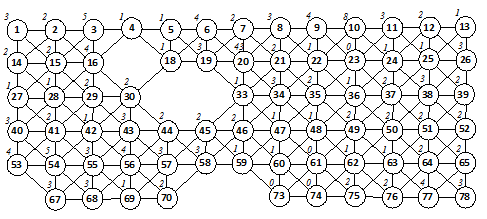
\includegraphics[angle=0,scale=1.25]{Figures/Laub/Gartengraph_Beispiel.png}}
\captionof{figure}{Beispiel für einen Garten in Graphendarstellung}
\label{Beispiel_Gartengraph}
\end{minipage}
\end{center}

\phantom \\
\noindent Es werde der Einfachheit halber angenommen, dass sämtliche Kanten mit 1 bewertet sind und die dementsprechend ermittelten Entfernungen zwischen den Knoten in der zugehörigen Matrix $D=(d_{ij})$ hinterlegt sind ($i=1,\dots,6; j=1,\dots,13$). Zudem wird das südwestliche Feld als Kompostfeld festgelegt: $K=66 \equiv (6,1)$. Die Entfernung $d_{a,K}$ von den Knoten $a$ zum Kompostfeld seien ebenfalls hinterlegt; dazu werde gesetzt: $d_{53,K}=d_{54,K}=d_{67,K}=1$. Als Anfangsfeld für den Harkprozess wird der Knoten 1 bestimmt. Zudem wird von einer konstanten Kapazitätsfunktion $\overline{M}$ ausgegangen und $\overline{M}(a)=20$ für alle $a \in V$ festgelegt. Für die Transportkapazität gelte: $\overline{T} \geq 20$; somit wird zu jedem Hub nur \textit{eine} Pendeltour benötigt.\footnote{Einsparungsmöglichkeiten durch Sammeltouren werden in \ref{Beispiel_Erläuterungen} diskutiert.}\\
\\
Jede Ergebnisdarstellung besteht aus der jeweiligen Nachfolgerfunktion $s$ in ausgerichteter Form und der Visualisierung des Harkprozesses, wobei die Pfeile die Harkrichtungen angeben, die entstandenen Cluster farbig hervorgehoben sind und in den Hubfeldern die kumulierten Laubharkmengen angegeben sind.

\section{Zickzack-Strategien am Beispiel}\label{sec_Zickzack}
%\noindent \textbf{\underline{Einfache Zickzack-Strategie am Beispiel}}\label{Zickzack_einfach}

\subsection{Einfache Zickzack-Strategie}\label{Zickzack_einfach}
\noindent Die \textit{einfache Zickzack-Strategie} liefert den folgenden Harkplan (Abb. \ref{Beispiel_Gartenmatrix_Zickzack}) mit zulässiger Nachfolgerfunktion $s$: 

\begin{center}
\begin{minipage}{\textwidth}
\renewcommand{\arraystretch}{1.2}
%\begin{table}[H]
%\caption{Ausgerichtete Nachfolgerfunktion zur einfachen Zickzack-Strategie am Beispiel}
%\centering 
\begin{scriptsize}
\begin{tabular}{|c|*{24}{|p{.15cm}}|}
\hline
$a$&1&2&3&4&5&6&\cellcolor{gray!25!white}7&8&9&10&11&\cellcolor{gray!25!white}12&13&26&25&24&23&22&21&20&19&\cellcolor{gray!25!white}18&16&15 \\
\hline
$s(a)$&2&3&4&5&6&7&\cellcolor{gray!25!white}7&9&10&11&12&\cellcolor{gray!25!white}12&26&25&24&23&22&21&20&19&18&\cellcolor{gray!25!white}18&15&14\\
\hline \hline
$a$&14&27&28&29&\cellcolor{gray!25!white}30&33&34&35&36&37&38&39&52&51&\cellcolor{gray!25!white}50&49&48&47&46&45&44&43&42&41\\
\hline
$s(a)$&27&28&29&30&\cellcolor{gray!25!white}30&34&35&36&37&38&39&52&51&50&\cellcolor{gray!25!white}50&48&47&46&45&44&43&42&41&40\\
\hline \hline
$a$&\cellcolor{gray!25!white}40&53&54&55&56&\cellcolor{gray!25!white}57&58&59&60&61&62&63&64&65&78&77&\cellcolor{gray!25!white}76&75&74&\cellcolor{gray!25!white}73&70&69&68&\cellcolor{gray!25!white}67\\
\hline
$s(a)$&\cellcolor{gray!25!white}40&54&55&56&57&\cellcolor{gray!25!white}57&59&60&61&62&63&64&65&78&77&76&\cellcolor{gray!25!white}76&74&73&\cellcolor{gray!25!white}73&69&68&67&\cellcolor{gray!25!white}67\\
\hline
\end{tabular}
\label{Beispiel_HF_Zickzack_einfach}
\end{scriptsize} 
%\end{table}
\renewcommand{\arraystretch}{1}
%\end{minipage}
%\end{center}

%\begin{center}
%\begin{minipage}{\textwidth}
\renewcommand{\arraystretch}{1.4}
\begin{table}[H]
\centering 
\begin{scriptsize}
\begin{tabular}{|>{}c|>{}c|>{}c|>{}c|>{}c|>{}c|>{}c|>{}c|>{}c|>{}c|>{}c|>{}c|>{}c|}
\hline
\cellcolor{red!15!white}$\rightarrow$&\cellcolor{red!15!white}$\rightarrow$&\cellcolor{red!15!white}$\rightarrow$&\cellcolor{red!15!white}$\rightarrow$&\cellcolor{red!15!white}$\rightarrow$&\cellcolor{red!15!white}$\rightarrow$&\cellcolor{red!15!white}\bf{18}&\cellcolor{green!15!white}
$\rightarrow$&\cellcolor{green!15!white}$\rightarrow$&\cellcolor{green!15!white}$\rightarrow$&\cellcolor{green!15!white}$\rightarrow$&\cellcolor{green!15!white}\bf{20}&\cellcolor{yellow!15!white}$\downarrow$\\
\hline
\cellcolor{green!15!white}$\downarrow$&\cellcolor{green!15!white}$\leftarrow$&\cellcolor{green!15!white}$\leftarrow$&\cellcolor{gray!50!white} &\cellcolor{yellow!15!white}\bf{17}&
\cellcolor{yellow!15!white}$\leftarrow$&\cellcolor{yellow!15!white}$\leftarrow$&\cellcolor{yellow!15!white}$\leftarrow$&\cellcolor{yellow!15!white}$\leftarrow$&\cellcolor{yellow!15!white}$\leftarrow$&\cellcolor{yellow!15!white}$\leftarrow$&\cellcolor{yellow!15!white}$\leftarrow$&\cellcolor{yellow!15!white}$\leftarrow$ \\
\hline
\cellcolor{green!15!white}$\rightarrow$&\cellcolor{green!15!white}$\rightarrow$&\cellcolor{green!15!white}$\rightarrow$&\cellcolor{green!15!white}\bf{14}&\cellcolor{gray!50!white} &\cellcolor{gray!50!white} &\cellcolor{blue!15!white}$\rightarrow$&\cellcolor{blue!15!white}$\rightarrow$&\cellcolor{blue!15!white}$\rightarrow$&\cellcolor{blue!15!white}$\rightarrow$&\cellcolor{blue!15!white}$\rightarrow$&\cellcolor{blue!15!white}$\rightarrow$&\cellcolor{blue!15!white}$\downarrow$ \\
\hline
\cellcolor{red!15!white}\bf{19}&\cellcolor{red!15!white}$\leftarrow$&\cellcolor{red!15!white}$\leftarrow$&\cellcolor{red!15!white}$\leftarrow$&\cellcolor{red!15!white}$\leftarrow$&\cellcolor{red!15!white}$\leftarrow$&\cellcolor{red!15!white}$\leftarrow$&\cellcolor{red!15!white}$\leftarrow$
&\cellcolor{red!15!white}$\leftarrow$&\cellcolor{red!15!white}$\leftarrow$&\cellcolor{blue!15!white}\bf{20}&\cellcolor{blue!15!white}$\leftarrow$&\cellcolor{blue!15!white}$\leftarrow$ \\
\hline
\cellcolor{yellow!15!white}$\rightarrow$&\cellcolor{yellow!15!white}$\rightarrow$&\cellcolor{yellow!15!white}$\rightarrow$&\cellcolor{yellow!15!white}$\rightarrow$&\cellcolor{yellow!15!white}\bf{19}&\cellcolor{green!15!white}$\rightarrow$&\cellcolor{green!15!white}$\rightarrow$
&\cellcolor{green!15!white}$\rightarrow$&\cellcolor{green!15!white}$\rightarrow$&\cellcolor{green!15!white}$\rightarrow$&\cellcolor{green!15!white}$\rightarrow$&\cellcolor{green!15!white}$\rightarrow$&\cellcolor{green!15!white}$\downarrow$\\
\hline
\cellcolor{gray!50!white} &\cellcolor{blue!15!white}\bf{9}&\cellcolor{blue!15!white}$\leftarrow$&\cellcolor{blue!15!white}$\leftarrow$&\cellcolor{blue!15!white}$\leftarrow$&\cellcolor{gray!50!white} &\cellcolor{gray!50!white} &\cellcolor{yellow!15!white}\bf{2}&\cellcolor{yellow!15!white}$\leftarrow$&\cellcolor{yellow!15!white}$\leftarrow$&\cellcolor{green!15!white}\bf{20}&\cellcolor{green!15!white}$\leftarrow$&\cellcolor{green!15!white}$\leftarrow$ \\
\hline
\end{tabular}
\captionof{figure}{Harkplan durch einfache Zickzack-Strategie am Beispiel}
\label{Beispiel_Gartenmatrix_Zickzack}
\end{scriptsize} 
\end{table}
\renewcommand{\arraystretch}{1}
\end{minipage}
\end{center}

\phantom \\
\noindent Die gesamte Laubmenge des Gartens in Höhe von 158 [ME] werden dabei auf 10 Hubs zusammengeharkt. Dabei entsteht gemäß (\ref{Harkaufwandsformel_1}) ein produktiver Harkaufwand von $HA_{\Sigma}(s)=517$ [ZE] bei Parametersetzung $\alpha_H = 1$ [ZE/ME].\footnote{Diese Standardsetzung für $\alpha_H$ erfolgt insofern o.B.d.A., da lediglich das Verhältnis zu den beiden anderen Parametern $\alpha_W$ und $\alpha_T$ das Gütemaß für eine Harkstrategie entscheidend beeinflusst.} Gemäß (\ref{Wegeaufwandsformel_1}) ergibt sich als Summe der unproduktiven Wege zu $W(s)=14$ [LE], die durch Gewichtung mit dem Wegeparameter $\alpha_W$ gemäß (\ref{Wegeaufwandsformel_2}) einen unproduktiven Wegeaufwand $WA_{\Sigma}(s) = 14 \cdot \alpha_W$ [ZE] ergibt.\footnote{Hierbei ist zu beachten, dass die Übergänge von einem erreichten Hub zur nächsten Harkquelle hierbei in Zickzack-Richtung erfolgt. Bei Beachtung des "`Nächster Nachfolger"'-Prinzips ergäben sich 18 [LE].} Für die Bestimmung des Transportaufwandes sind der Einfachheit halber ausschließlich Pendeltouren zwischen den Hubs und dem Kompostfeld zugelassen, deren Einzelaufwände gemäß (\ref{Transportaufwandsformel_1}) sich zum Gesamttransportaufwand $TA_{\Sigma} = 116\cdot \alpha_T$ [ZE] aufsummieren (vgl. (\ref{Transportaufwandsformel_5})). Demnach ergibt sich aus der einfachen Zickzack-Strategie ein Gesamtaufwand von $K(s) = 517 + 14 \cdot \alpha_W + 116\cdot \alpha_T$ [ZE]. \\
\\
Durch Anwendung von \textit{Hubzentrierung}\footnote{Hierbei wird primär das \textit{Maximalmengen-Kriterium} (\ref{Maximalmengenkriterium}), sekundär das \textit{Median-Kriterium} (\ref{Mediankriterium}) und tertiär das \textit{Indexkriterium} (\ref{Indexkriterium}) angewendet; vgl. Abschn. \ref{section_Hubzentrierung}.} und \textit{Hubausrichtung} ergibt sich der folgende Harkprozess (Abb. \ref{Beispiel_Gartenmatrix_Zickzack_mit_Hubausrichtung}) mit zugehöriger Nachfolgerfuktion $s$, wobei sich der zugehörige Gesamtaufwand auf $K(s) = 254 + 47 \cdot \alpha_W + 114 \cdot \alpha_T$ [ZE] deutlich verringert, zumal $\alpha_W \leq 1$ angenommen werden kann.


\begin{center}
\begin{minipage}{\textwidth}
\renewcommand{\arraystretch}{1.2}
%\begin{table}[H]
%\caption{Ausgerichtete Nachfolgerfunktion nach Hubausrichtung am Beispiel}
%\centering 
\begin{scriptsize}
\begin{tabular}{|c|*{24}{|p{.15cm}}|}
\hline
$a$&1&2&14&27&15&28&29&30&\cellcolor{gray!25!white}16&18&19&7&6&5&4&\cellcolor{gray!25!white}3&40&41&42&57&56&55&53&\cellcolor{gray!25!white}54 \\
\hline
$s(a)$&2&3&15&15&16&16&16&16&\cellcolor{gray!25!white}16&19&20&6&5&4&3&\cellcolor{gray!25!white}3&41&42&43&56&55&54&54&\cellcolor{gray!25!white}54\\
\hline \hline
$a$&67&70&69&\cellcolor{gray!25!white}68&58&59&60&61&62&63&64&65&76&78&\cellcolor{gray!25!white}77&49&48&47&46&45&44&\cellcolor{gray!25!white}43&33&34\\
\hline
$s(a)$&68&69&68&\cellcolor{gray!25!white}68&59&60&61&62&63&77&77&77&77&77&\cellcolor{gray!25!white}77&48&47&46&45&44&43&\cellcolor{gray!25!white}43&34&35\\
\hline \hline
$a$&35&36&37&26&11&8&9&\cellcolor{gray!25!white}10&12&13&25&24&23&22&21&\cellcolor{gray!25!white}20&50&39&51&52&\cellcolor{gray!25!white}38&73&74&\cellcolor{gray!25!white}75\\
\hline
$s(a)$&36&37&38&25&10&9&10&\cellcolor{gray!25!white}10&24&25&24&23&22&21&20&\cellcolor{gray!25!white}20&38&38&38&38&\cellcolor{gray!25!white}38&74&75&\cellcolor{gray!25!white}75\\
\hline
\end{tabular}
\label{Beispiel_HF_Zickzack_mit_Hubausrichtung}
\end{scriptsize} 
%\end{table}
\renewcommand{\arraystretch}{1}
%\end{minipage}
%\end{center}

%\begin{center}
%\begin{minipage}{\textwidth}
\renewcommand{\arraystretch}{1.4}
\begin{table}[H]
\centering 
\begin{scriptsize}
\begin{tabular}{|>{}c|>{}c|>{}c|>{}c|>{}c|>{}c|>{}c|>{}c|>{}c|>{}c|>{}c|>{}c|>{}c|}
\hline
\cellcolor{red!15!white}$\rightarrow$&\cellcolor{red!15!white}$\rightarrow$&\cellcolor{red!15!white}\bf{18}&\cellcolor{red!15!white}$\leftarrow$&\cellcolor{red!15!white}$\leftarrow$&\cellcolor{red!15!white}$\leftarrow$&\cellcolor{red!15!white}$\leftarrow$&
\cellcolor{green!15!white}$\rightarrow$&\cellcolor{green!15!white}$\rightarrow$&\cellcolor{green!15!white}$\rightarrow$&\cellcolor{green!15!white}\bf{20}&\cellcolor{green!15!white}$\leftarrow$&\cellcolor{yellow!15!white}$\swarrow$\\
\hline
\cellcolor{green!15!white}$\rightarrow$&\cellcolor{green!15!white}$\rightarrow$&\cellcolor{green!15!white}\bf{14}&\cellcolor{gray!50!white} &\cellcolor{yellow!15!white}$\rightarrow$&\cellcolor{yellow!15!white}$\rightarrow$& \cellcolor{yellow!15!white}\bf{17}&\cellcolor{yellow!15!white}$\leftarrow$&\cellcolor{yellow!15!white}$\leftarrow$&\cellcolor{yellow!15!white}$\leftarrow$&\cellcolor{yellow!15!white}$\leftarrow$&\cellcolor{yellow!15!white}$\leftarrow$&\cellcolor{yellow!15!white}$\leftarrow$ \\
\hline
\cellcolor{green!15!white}$\nearrow$&\cellcolor{green!15!white}$\nearrow$&\cellcolor{green!15!white}$\uparrow$&\cellcolor{green!15!white}$\nwarrow$&\cellcolor{gray!50!white} &\cellcolor{gray!50!white} &\cellcolor{blue!15!white}$\rightarrow$&\cellcolor{blue!15!white}$\rightarrow$&\cellcolor{blue!15!white}$\rightarrow$&\cellcolor{blue!15!white}$\rightarrow$&\cellcolor{blue!15!white}$\rightarrow$&\cellcolor{blue!15!white}\bf{20}&\cellcolor{blue!15!white}$\leftarrow$ \\
\hline
\cellcolor{red!15!white}$\rightarrow$&\cellcolor{red!15!white}$\rightarrow$&\cellcolor{red!15!white}$\rightarrow$&\cellcolor{red!15!white}\bf{19}&\cellcolor{red!15!white}$\leftarrow$&\cellcolor{red!15!white}$\leftarrow$&\cellcolor{red!15!white}$\leftarrow$&\cellcolor{red!15!white}$\leftarrow$
&\cellcolor{red!15!white}$\leftarrow$&\cellcolor{red!15!white}$\leftarrow$&\cellcolor{blue!15!white}$\nearrow$&\cellcolor{blue!15!white}$\uparrow$&\cellcolor{blue!15!white}$\nwarrow$ \\
\hline
\cellcolor{yellow!15!white}$\rightarrow$&\cellcolor{yellow!15!white}\bf{19}&\cellcolor{yellow!15!white}$\leftarrow$&\cellcolor{yellow!15!white}$\leftarrow$&\cellcolor{yellow!15!white}$\leftarrow$&\cellcolor{green!15!white}$\rightarrow$&\cellcolor{green!15!white}$\rightarrow$
&\cellcolor{green!15!white}$\rightarrow$&\cellcolor{green!15!white}$\rightarrow$&\cellcolor{green!15!white}$\rightarrow$&\cellcolor{green!15!white}$\searrow$&\cellcolor{green!15!white}$\downarrow$&\cellcolor{green!15!white}$\swarrow$\\
\hline
\cellcolor{gray!50!white} &\cellcolor{blue!15!white}$\rightarrow$&\cellcolor{blue!15!white}\bf{9}&\cellcolor{blue!15!white}$\leftarrow$&\cellcolor{blue!15!white}$\leftarrow$&\cellcolor{gray!50!white} &\cellcolor{gray!50!white} &\cellcolor{yellow!15!white}$\rightarrow$&\cellcolor{yellow!15!white}$\rightarrow$&\cellcolor{yellow!15!white}\bf{2}&\cellcolor{green!15!white}$\rightarrow$&\cellcolor{green!15!white}\bf{20}&\cellcolor{green!15!white}$\leftarrow$ \\
\hline
\end{tabular}
\captionof{figure}{Harkplan durch einfache Zickzack-Strategie nach Hubausrichtung am Beispiel}
\label{Beispiel_Gartenmatrix_Zickzack_mit_Hubausrichtung}
\end{scriptsize} 
\end{table}
\renewcommand{\arraystretch}{1}
\end{minipage}
\end{center}

%\phantom \\
\subsection{Unterteilte Zickzack-Strategie}\label{Zickzack_unterteilt}
%\noindent \textbf{\underline{Unterteilte Zickzack-Strategie am Beispiel}} \label{Zickzack_unterteilt}

\noindent Die obige Gartenmatrix wird nun in drei Teilmatrizen unterteilt: $n_1 = 4, n_2 = 10$.
Die Anwendung der \textit{unterteilten Zickzack-Strategie} führt zu folgendem Harkprozess:

\begin{center}
\begin{minipage}{\textwidth}
\renewcommand{\arraystretch}{1.2}
%\begin{table}[H]
%\caption{Ausgerichtete Nachfolgerfunktion für unterteilte Zickzack-Strategie am Beispiel}
%\centering 
\begin{scriptsize}
\begin{tabular}{|c|*{24}{|p{.15cm}}|}
\hline
$a$&1&2&3&\cellcolor{gray!25!white}4&16&15&14&27&28&29&30&43&42&\cellcolor{gray!25!white}41&40&53&54&55&\cellcolor{gray!25!white}56&69&68&\cellcolor{gray!25!white}67&5&6 \\
\hline
$s(a)$&2&3&4&\cellcolor{gray!25!white}4&15&14&27&28&29&30&43&42&41&\cellcolor{gray!25!white}41&53&54&55&56&\cellcolor{gray!25!white}56&68&67&\cellcolor{gray!25!white}67&6&7\\
\hline \hline
$a$&7&8&9&22&\cellcolor{gray!25!white}21&20&19&\cellcolor{gray!25!white}18&33&34&35&48&47&46&45&44&57&\cellcolor{gray!25!white}58&59&60&61&74&\cellcolor{gray!25!white}73&10\\
\hline
$s(a)$&8&9&22&21&\cellcolor{gray!25!white}21&19&18&\cellcolor{gray!25!white}18&34&35&48&47&46&45&44&57&58&\cellcolor{gray!25!white}58&60&61&74&73&\cellcolor{gray!25!white}73&11\\
\hline \hline
$a$&11&12&13&26&25&24&23&\cellcolor{gray!25!white}36&37&38&39&52&51&50&49&62&63&\cellcolor{gray!25!white}64&65&78&77&76&\cellcolor{gray!25!white}75&\cellcolor{gray!25!white}70\\
\hline
$s(a)$&12&13&26&25&24&23&36&\cellcolor{gray!25!white}36&38&39&52&51&50&49&62&63&64&\cellcolor{gray!25!white}64&78&77&76&75&\cellcolor{gray!25!white}75&\cellcolor{gray!25!white}70\\
\hline
\end{tabular}
\label{Beispiel_HF_Zickzack_unterteilt}
\end{scriptsize} 
%\end{table}
\renewcommand{\arraystretch}{1}
%\end{minipage}
%\end{center}

%\begin{center}
%\begin{minipage}{\textwidth}
\renewcommand{\arraystretch}{1.4}
\begin{table}[H]
\centering 
\begin{scriptsize}
\begin{tabular}{|>{}c|>{}c|>{}c|>{}c||>{}c|>{}c|>{}c|>{}c|>{}c||>{}c|>{}c|>{}c|>{}c|}
\hline
\cellcolor{red!15!white}$\rightarrow$&\cellcolor{red!15!white}$\rightarrow$&\cellcolor{red!15!white}$\rightarrow$\cellcolor{red!15!white}&\cellcolor{red!15!white}\bf{11}&
\cellcolor{green!15!white}$\rightarrow$&\cellcolor{green!15!white}$\rightarrow$&\cellcolor{green!15!white}$\rightarrow$&\cellcolor{green!15!white}$\rightarrow$&\cellcolor{green!15!white}$\downarrow$&
\cellcolor{red!15!white}$\rightarrow$&\cellcolor{red!15!white}$\rightarrow$&\cellcolor{red!15!white}$\rightarrow$&\cellcolor{red!15!white}$\downarrow$\\
\hline
\cellcolor{green!15!white}$\downarrow$&\cellcolor{green!15!white}$\leftarrow$&\cellcolor{green!15!white}$\leftarrow$&\cellcolor{gray!50!white} &
\cellcolor{yellow!15!white}\bf{8}&\cellcolor{yellow!15!white}$\leftarrow$&\cellcolor{yellow!15!white}$\leftarrow$&\cellcolor{green!15!white}\bf{17}&\cellcolor{green!15!white}$\leftarrow$&
\cellcolor{red!15!white}$\downarrow$&\cellcolor{red!15!white}$\leftarrow$&\cellcolor{red!15!white}$\leftarrow$&\cellcolor{red!15!white}$\leftarrow$ \\
\hline
\cellcolor{green!15!white}$\rightarrow$&\cellcolor{green!15!white}$\rightarrow$&\cellcolor{green!15!white}$\rightarrow$&\cellcolor{green!15!white}$\downarrow$&
\cellcolor{gray!50!white} &\cellcolor{gray!50!white} &\cellcolor{blue!15!white}$\rightarrow$ &\cellcolor{blue!15!white}$\rightarrow$ &\cellcolor{blue!15!white}$\downarrow$ &\cellcolor{red!15!white}\bf{20}&\cellcolor{green!15!white}$\rightarrow$ &\cellcolor{green!15!white}$\rightarrow$ &\cellcolor{green!15!white}$\downarrow$ \\
\hline
\cellcolor{red!15!white}$\downarrow$&\cellcolor{green!15!white}\bf{20}&\cellcolor{green!15!white}$\leftarrow$&\cellcolor{green!15!white}$\leftarrow$&
\cellcolor{blue!15!white}$\downarrow$&\cellcolor{blue!15!white}$\leftarrow$&\cellcolor{blue!15!white}$\leftarrow$&\cellcolor{blue!15!white}$\leftarrow$&\cellcolor{blue!15!white}$\leftarrow$ 
&\cellcolor{green!15!white}$\downarrow$ &\cellcolor{green!15!white}$\leftarrow$&\cellcolor{green!15!white}$\leftarrow$ &\cellcolor{green!15!white}$\leftarrow$ \\
\hline
\cellcolor{red!15!white}$\rightarrow$&\cellcolor{red!15!white}$\rightarrow$&\cellcolor{red!15!white}$\rightarrow$&\cellcolor{red!15!white}\bf{19}&
\cellcolor{blue!15!white}$\rightarrow$&\cellcolor{blue!15!white}\bf{20}&\cellcolor{red!15!white}$\rightarrow$&\cellcolor{red!15!white}$\rightarrow$&\cellcolor{red!15!white}$\downarrow$ &\cellcolor{green!15!white}$\rightarrow$&\cellcolor{green!15!white}$\rightarrow$&\cellcolor{green!15!white}\bf{19}&\cellcolor{yellow!15!white}$\downarrow$\\
\hline
\cellcolor{gray!50!white} &\cellcolor{yellow!15!white}\bf{7}&\cellcolor{yellow!15!white}$\leftarrow$&\cellcolor{yellow!15!white}$\leftarrow$&
\cellcolor{green!15!white}\bf{2}&\cellcolor{gray!50!white} &\cellcolor{gray!50!white} &\cellcolor{red!15!white}\bf{2}&\cellcolor{red!15!white}$\leftarrow$& \cellcolor{yellow!15!white}\bf{13}&\cellcolor{yellow!15!white}$\leftarrow$&\cellcolor{yellow!15!white}$\leftarrow$&\cellcolor{yellow!15!white}$\leftarrow$ \\
\hline
\end{tabular}
\captionof{figure}{Harkplan durch unterteilte Zickzack-Strategie am Beispiel}
\label{Beispiel_Gartenmatrix_Zickzack_unterteilt}
\end{scriptsize} 
\end{table}
\renewcommand{\arraystretch}{1}
\end{minipage}
\end{center}

\phantom \\
\noindent Die gesamte Laubmenge des Gartens in Höhe von 158 [ME] werden dabei auf 12 Hubs zusammengeharkt. Unter denselben Setzungen wie beim einfachen Zickzack-Harken entsteht nun ein Harkaufwand von $HA_{\Sigma}(s)=570$ [ZE], ein Wegeaufwand $WA_{\Sigma}(s) = 19 \cdot \alpha_W$ [ZE] und ein Transportaufwand von $TA_{\Sigma} = 134\cdot \alpha_T$ [ZE], insgesamt also ein Gesamtaufwand von $K(s) = 570 + 19 \cdot \alpha_W + 134\cdot \alpha_T$ [ZE]. \\ 
\\
Da alle Teilaufwände bei obiger Lösung größer als beim einfachen Zickzack-Harken sind (vgl. Abb.  \ref{Beispiel_Gartenmatrix_Zickzack}), ist auch der Gesamtaufwand größer, und zwar unabhängig von den Harkparametern.\\
\\
\noindent Durch Hubzentrierung und -ausrichtung dieser Startlösung (vgl. Abb. \ref{Beispiel_Gartenmatrix_Zickzack_unterteilt_Hubausrichtung}) erhält man eine deutlich verbesserte Lösung: 
$K(s) = 174 + 68 \cdot \alpha_W + 144\cdot \alpha_T$. Unter der Annahme $\alpha_W \leq 1$ ist diese Lösung im Vergleich zur ebenfalls zentrierten und hubausgerichteten Lösung bei einfacher Zickzack-Strategie (vgl. Abb. \ref{Beispiel_Gartenmatrix_Zickzack_mit_Hubausrichtung}) dann schlechter, wenn in erwa der Parameter $\alpha_T > 2,5$ ausfällt. 

\begin{center}
\begin{minipage}{\textwidth}
\renewcommand{\arraystretch}{1.2}
%\begin{table}[H]
%\caption{Ausgerichtete Nachfolgerfunktion für unterteilte Zickzack-Strategie nach Hubzentrierung uns -ausrichtung am Beispiel}
%\centering 
\begin{scriptsize}
\begin{tabular}{|c|*{24}{|p{.15cm}}|}
\hline
$a$&1&2&4&\cellcolor{gray!25!white}3&5&6&7&8&21&22&\cellcolor{gray!25!white}9&24&25&36&23&35&33&45&44&57&30&14&27&15 \\
\hline
$s(a)$&2&3&3&\cellcolor{gray!25!white}3&6&7&8&9&9&9&\cellcolor{gray!25!white}9&10&11&23&10&34&45&58&58&58&16&15&15&16\\
\hline \hline
$a$&18&19&\cellcolor{gray!25!white}20&47&48&34&46&\cellcolor{gray!25!white}58&43&29&40&41&42&28&\cellcolor{gray!25!white}16&53&67&56&55&\cellcolor{gray!25!white}54&69&\cellcolor{gray!25!white}68&73&61\\
\hline
$s(a)$&19&20&\cellcolor{gray!25!white}20&46&34&46&58&\cellcolor{gray!25!white}58&29&16&54&28&28&16&\cellcolor{gray!25!white}16&54&68&55&54&\cellcolor{gray!25!white}54&68&\cellcolor{gray!25!white}68&59&60\\
\hline \hline
$a$&74&60&\cellcolor{gray!25!white}59&46&37&26&13&12&11&\cellcolor{gray!25!white}10&39&51&52&62&63&64&50&\cellcolor{gray!25!white}38&65&78&75&76&\cellcolor{gray!25!white}77&\cellcolor{gray!25!white}70\\
\hline
$s(a)$&60&59&\cellcolor{gray!25!white}59&37&38&12&12&11&10&\cellcolor{gray!25!white}10&38&38&38&50&50&50&38&\cellcolor{gray!25!white}38&77&77&76&77&\cellcolor{gray!25!white}77&\cellcolor{gray!25!white}70\\
\hline
\end{tabular}
\label{Beispiel_HF_Zickzack_unterteilt_mit_Hubausrichtung}
\end{scriptsize} 
%\end{table}
\renewcommand{\arraystretch}{1}
%\end{minipage}
%\end{center}

%\begin{center}
%\begin{minipage}{\textwidth}
\renewcommand{\arraystretch}{1.4}
\begin{table}[H]
\centering 
\begin{scriptsize}
\begin{tabular}{|>{}c|>{}c|>{}c|>{}c||>{}c|>{}c|>{}c|>{}c|>{}c||>{}c|>{}c|>{}c|>{}c|}
\hline
\cellcolor{red!15!white}$\rightarrow$&\cellcolor{red!15!white}$\rightarrow$&\cellcolor{red!15!white}\bf{11}&\cellcolor{red!15!white}$\leftarrow$&
\cellcolor{green!15!white}$\rightarrow$&\cellcolor{green!15!white}$\rightarrow$&\cellcolor{green!15!white}$\rightarrow$&\cellcolor{green!15!white}$\rightarrow$&\cellcolor{green!15!white}\bf{17}&
\cellcolor{red!15!white}\bf{20}&\cellcolor{red!15!white}$\leftarrow$&\cellcolor{red!15!white}$\leftarrow$&\cellcolor{red!15!white}$\leftarrow$\\
\hline
\cellcolor{green!15!white}$\rightarrow$&\cellcolor{green!15!white}$\rightarrow$&\cellcolor{green!15!white}\bf{20}&\cellcolor{gray!50!white} &
\cellcolor{yellow!15!white}$\rightarrow$&\cellcolor{yellow!15!white}$\rightarrow$&\cellcolor{yellow!15!white}\bf{8}&\cellcolor{green!15!white}$\nearrow$&\cellcolor{green!15!white}$\uparrow$&
\cellcolor{red!15!white}$\uparrow$&\cellcolor{red!15!white}$\nwarrow$&\cellcolor{red!15!white}$\nwarrow$&\cellcolor{red!15!white}$\nwarrow$ \\
\hline
\cellcolor{green!15!white}$\nearrow$&\cellcolor{green!15!white}$\nearrow$&\cellcolor{green!15!white}$\uparrow$&\cellcolor{green!15!white}$\nwarrow$&
\cellcolor{gray!50!white} &\cellcolor{gray!50!white} &\cellcolor{blue!15!white}$\swarrow$&\cellcolor{blue!15!white}$\swarrow$&\cellcolor{blue!15!white}$\leftarrow$ &\cellcolor{red!15!white}$\uparrow$&\cellcolor{green!15!white}$\rightarrow$ &\cellcolor{green!15!white}\bf{19}&\cellcolor{green!15!white}$\leftarrow$ \\
\hline
\cellcolor{red!15!white}$\searrow$&\cellcolor{green!15!white}$\uparrow$&\cellcolor{green!15!white}$\nwarrow$&\cellcolor{green!15!white}$\nwarrow$&
\cellcolor{blue!15!white}$\searrow$&\cellcolor{blue!15!white}$\downarrow$&\cellcolor{blue!15!white}$\swarrow$&\cellcolor{blue!15!white}$\leftarrow$&\cellcolor{blue!15!white}$\nwarrow$ 
&\cellcolor{green!15!white}$\nearrow$&\cellcolor{green!15!white}$\nearrow$&\cellcolor{green!15!white}$\uparrow$&\cellcolor{green!15!white}$\nwarrow$ \\
\hline
\cellcolor{red!15!white}$\rightarrow$&\cellcolor{red!15!white}\bf{19}&\cellcolor{red!15!white}$\leftarrow$&\cellcolor{red!15!white}$\leftarrow$&
\cellcolor{blue!15!white}$\rightarrow$&$\cellcolor{blue!15!white}\bf{20}$&\cellcolor{red!15!white}\bf{2}&\cellcolor{red!15!white}$\leftarrow$&\cellcolor{red!15!white}$\leftarrow$ &\cellcolor{green!15!white}$\nearrow$&\cellcolor{green!15!white}$\uparrow$&\cellcolor{green!15!white}$\nwarrow$&\cellcolor{yellow!15!white}$\swarrow$\\
\hline
\cellcolor{gray!50!white}&\cellcolor{yellow!15!white}$\rightarrow$&\cellcolor{yellow!15!white}\bf{7}&\cellcolor{yellow!15!white}$\leftarrow$&
\cellcolor{green!15!white}\bf{2}&\cellcolor{gray!50!white}&\cellcolor{gray!50!white}&\cellcolor{red!15!white}$\nwarrow$&\cellcolor{red!15!white}$\nwarrow$& \cellcolor{yellow!15!white}$\rightarrow$&\cellcolor{yellow!15!white}$\rightarrow$&\cellcolor{yellow!15!white}\bf{13}&\cellcolor{yellow!15!white}$\leftarrow$ \\
\hline
\end{tabular}
\captionof{figure}{Harkplan durch unterteilte Zickzack-Strategie nach Hubzentrierung und -ausrichtung am Beispiel}
\label{Beispiel_Gartenmatrix_Zickzack_unterteilt_Hubausrichtung}
\end{scriptsize} 
\end{table}
\renewcommand{\arraystretch}{1}
\end{minipage}
\end{center}



\section{Clusterorientiertes Konstruktionsverfahren am Beispiel} \label{Beispiel Clusterorientiertes Verfahren}
%\textbf{\underline{Clusterorientiertes Konstruktionsverfahren am Beispiel}} \label{Beispiel Clusterorientiertes Verfahren}

\noindent Zur obigen Gartenmatrix und unter den angegebenen Bedingungen entsteht der folgende Harkplan (Abb. \ref{Beispiel_Harkplan_CO_NW}) durch Anwendung des \textit{clusterorientierten Konstruktionsverfahrens} (vgl. Abschn. \ref{section_Clusterorientiertes_Konstruktionsverfahren}). Die Ausrichtung bei der Bestimmung neu aufzunehmender Knoten erfolgt in Ausrichtung auf die Nordwestecke, die auch Ausgangspunkt des Clusterbildungsprozesses darstellt. Somit kommt ausschließlich das Indexkriterium zum Einsatz. Nach der Bestimmung der Cluster werden diese einzeln einer Hubzentrierung und -ausrichtung unterzogen (vgl. Abschn \ref{section_Hubzentrierung} bzw. Absch. \ref{section_Hubausrichtung}). 

\begin{center}
\begin{minipage}{\textwidth}
\renewcommand{\arraystretch}{1.1}
%\begin{table}[H]
%\caption{Nachfolgerfunktion durch clusterorientiertes Konstruktionsverfahren (NW-Orientierung) nach Hubausrichtung am Beispiel}
%\centering 
\begin{scriptsize}
\begin{tabular}{|c|*{24}{|p{.15cm}}|}
\hline
$a$&1&14&2&4&5&7&20&8&21&9&23&35&22&\cellcolor{gray!25!white}10&37&38&13&26&12&39&25&47&33&19 \\
\hline
$s(a)$&2&2&3&5&6&6&6&9&9&10&10&22&10&\cellcolor{gray!25!white}10&24&24&12&12&11&25&11&34&19&6\\
\hline \hline
$a$&16&27&28&15&\cellcolor{gray!25!white}3&40&42&30&18&\cellcolor{gray!25!white}6&43&29&41&53&\cellcolor{gray!25!white}54&67&55&44&57&45&59&60&70&58\\
\hline
$s(a)$&3&15&15&3&\cellcolor{gray!25!white}3&54&30&18&6&\cellcolor{gray!25!white}6&29&41&54&54&\cellcolor{gray!25!white}54&55&56&45&45&46&46&46&58&46\\
\hline \hline
$a$&46&\cellcolor{gray!25!white}34&49&50&51&62&75&63&65&\cellcolor{gray!25!white}78&52&64&76&\cellcolor{gray!25!white}77&74&73&61&48&36&24&\cellcolor{gray!25!white}11&69&68&\cellcolor{gray!25!white}56\\
\hline
$s(a)$&34&\cellcolor{gray!25!white}34&63&63&63&63&63&77&78&\cellcolor{gray!25!white}78&64&77&77&\cellcolor{gray!25!white}77&61&61&48&36&24&11&\cellcolor{gray!25!white}11&56&56&\cellcolor{gray!25!white}56\\
\hline
\end{tabular}
\label{Beispiel_CO_NW}
\end{scriptsize} 
%\end{table}
\renewcommand{\arraystretch}{1}
%\end{minipage}
%\end{center}

%\begin{center}
%\begin{minipage}{\textwidth}
\renewcommand{\arraystretch}{1.35}
\begin{table}[H]
\centering 
\begin{scriptsize}
\begin{tabular}{|>{}c|>{}c|>{}c|>{}c|>{}c|>{}c|>{}c|>{}c|>{}c|>{}c|>{}c|>{}c|>{}c|}
\hline
\cellcolor{red!15!white}$\rightarrow$&\cellcolor{red!15!white}$\rightarrow$&\cellcolor{red!15!white}\bf{20}&\cellcolor{green!15!white}$\rightarrow$&\cellcolor{green!15!white}$\rightarrow$&\cellcolor{green!15!white}\bf{20}&\cellcolor{green!15!white}$\leftarrow$&\cellcolor{blue!15!white}$\rightarrow$&\cellcolor{blue!15!white}$\rightarrow$&\cellcolor{blue!15!white}\bf{20}&\cellcolor{red!15!white}\bf{20}&\cellcolor{red!15!white}$\leftarrow$&$\cellcolor{red!15!white}\leftarrow$\\
\hline
\cellcolor{red!15!white}$\nearrow$&\cellcolor{red!15!white}$\nearrow$&\cellcolor{red!15!white}$\uparrow$&\cellcolor{gray!50!white} &
\cellcolor{green!15!white}$\nearrow$&\cellcolor{green!15!white}$\uparrow$&\cellcolor{green!15!white}$\nwarrow$&\cellcolor{blue!15!white}$\nearrow$&
\cellcolor{blue!15!white}$\nearrow$&\cellcolor{blue!15!white}$\uparrow$&\cellcolor{red!15!white}$\uparrow$&\cellcolor{red!15!white}$\nwarrow$&\cellcolor{red!15!white}$\nwarrow$ \\
\hline
\cellcolor{red!15!white}$\nearrow$&\cellcolor{red!15!white}$\uparrow$&\cellcolor{blue!15!white}$\swarrow$&\cellcolor{green!15!white}$\nearrow$&
\cellcolor{gray!50!white}&\cellcolor{gray!50!white}&\cellcolor{green!15!white}$\nwarrow$ &\cellcolor{yellow!15!white}\bf{20} &\cellcolor{blue!15!white}$\uparrow$ &\cellcolor{red!15!white}$\nearrow$&\cellcolor{red!15!white}$\uparrow$ &\cellcolor{red!15!white}$\nwarrow$ &\cellcolor{red!15!white}$\nwarrow$ \\
\hline
\cellcolor{blue!15!white}$\searrow$&\cellcolor{blue!15!white}$\downarrow$&\cellcolor{green!15!white}$\nearrow$&\cellcolor{blue!15!white}$\nwarrow$&\cellcolor{yellow!15!white}
$\rightarrow$&\cellcolor{yellow!15!white}$\rightarrow$&\cellcolor{yellow!15!white}$\nearrow$&\cellcolor{yellow!15!white}$\uparrow$&\cellcolor{red!15!white}$\nearrow$ 
&\cellcolor{green!15!white}$\searrow$ &\cellcolor{green!15!white}$\downarrow$&\cellcolor{green!15!white}$\swarrow$ &\cellcolor{green!15!white}$\swarrow$ \\
\hline
\cellcolor{blue!15!white}$\rightarrow$&\cellcolor{blue!15!white}\bf{19}&\cellcolor{red!15!white}$\rightarrow$&\cellcolor{red!15!white}\bf{14}&\cellcolor{yellow!15!white}
$\nearrow$&\cellcolor{yellow!15!white}$\nearrow$&\cellcolor{yellow!15!white}$\uparrow$&\cellcolor{yellow!15!white}$\nwarrow$&\cellcolor{red!15!white}$\uparrow$ &\cellcolor{green!15!white}$\rightarrow$&\cellcolor{green!15!white}$\searrow$&\cellcolor{green!15!white}$\downarrow$&\cellcolor{blue!15!white}$\downarrow$\\
\hline
\cellcolor{gray!50!white} &\cellcolor{red!15!white}$\nearrow$&\cellcolor{red!15!white}$\nearrow$&\cellcolor{red!15!white}$\uparrow$&
\cellcolor{yellow!15!white}$\nearrow$&\cellcolor{gray!50!white} &\cellcolor{gray!50!white} &\cellcolor{red!15!white}$\nearrow$&\cellcolor{red!15!white}$\uparrow$& \cellcolor{green!15!white}$\nearrow$&\cellcolor{green!15!white}$\rightarrow$&\cellcolor{green!15!white}\bf{20}&\cellcolor{blue!15!white}\bf{5} \\
\hline
\end{tabular}
\captionof{figure}{Harkplan durch clusterorientiertes Verfahren (NW-Orientierung) nach Hubausrichtung am Beispiel}
\label{Beispiel_Harkplan_CO_NW}
\end{scriptsize} 
\end{table}
\renewcommand{\arraystretch}{1}
\end{minipage}
\end{center}

\noindent Die gesamte Laubmenge des Gartens in Höhe von 158 [ME] werden dabei auf 9 Hubs zusammengeharkt. Unter denselben Setzungen wie bei den obigen Harkstrategien entsteht ein Harkaufwand von $HA_{\Sigma}(s)=196 \cdot \alpha_H$ [ZE], ein Wegeaufwand $WA_{\Sigma}(s) = 65 \cdot \alpha_W$ [ZE] und ein Transportaufwand von $TA_{\Sigma} = 126\cdot \alpha_T$ [ZE], insgesamt bei Setzung $\alpha_H = 1$ also ein Gesamtaufwand von $K(s) = 196 + 65 \cdot \alpha_W + 126\cdot \alpha_T$ [ZE].


%\noindent
\section{Huborientiertes Konstruktionsverfahren am Beispiel}\label{Beispiel Huborientiertes Verfahren}
%\textbf{\underline{Huborientiertes Konstruktionsverfahren am Beispiel}} \label{Beispiel Huborientiertes Verfahren}

\noindent Zur obigen Gartenmatrix und unter den angegebenen Bedingungen werden unterschiedliche Harkpläne nach dem \textit{huborientierten Konstruktionsverfahren} entwickelt (vgl. Abschn. \ref{section_Huborientiertes_Konstruktionsverfahren}): \\
\\
Zunächst wird bei der Knotenbestimmung für neue Hubs bzw. Harkvorgänger eine Tiefensuche (TS) vorgenommen. Dabei wird zum einen das Minimum-, zum zweiten das Maximummengen-Kriterium zur Auswahl der jeweiligen Harkvorgänger benutzt, wobei anschließend die Nachfolgerfunktionen auf die Hubs in den jeweiligen Clustern ausgerichtet werden (vgl. Abschn. \ref{section_Hubausrichtung}). Beim letzten Harkplan wird eine Breitensuche (BS) vorgenommen. Als Sekundärkriterium kommt jeweils das Indexkriterium zum Einsatz. 


\subsection{Huborientiertes Konstruktionsverfahren via Tiefensuche}
\label{Beispiel Huborientiertes Verfahren TS}

Bei der Auswahl der jeweiligen Harkvorgänger wird das Minimummengen-Kriterium benutzt, wobei 
der zuletzt aufgenommene Knoten als Ausgangspunkt für die weitere Knotensuche dient (Tiefensuche). Der daraus resultierende Harkplan ist in Abb. \ref{Beispiel_Harkplan_HO_Minimal} zu sehen:

\begin{center}
\begin{minipage}{\textwidth}
\renewcommand{\arraystretch}{1.1}
%\begin{table}[H]
%\caption{Nachfolgerfunktion durch huborientiertes Konstruktionsverfahren (TS) mit Minimalmengen-Kriterium am Beispiel}
%\centering 
\begin{scriptsize}
\begin{tabular}{|c|*{24}{|p{.15cm}}|}
\hline
$a$&\cellcolor{gray!25!white}1&29&15&40&41&42&28&27&14&2&18&5&4&\cellcolor{gray!25!white}3&30&43&68&67&\cellcolor{gray!25!white}53&69&55&\cellcolor{gray!25!white}54&44&45 \\
\hline
$s(a)$&\cellcolor{gray!25!white}1&15&14&54&54&28&27&14&2&3&5&4&3&\cellcolor{gray!25!white}3&43&55&67&53&\cellcolor{gray!25!white}53&55&54&\cellcolor{gray!25!white}54&45&46\\
\hline \hline
$a$&46&34&8&\cellcolor{gray!25!white}9&23&12&\cellcolor{gray!25!white}11&13&25&24&38&\cellcolor{gray!25!white}26&39&51&50&37&49&35&21&7&\cellcolor{gray!25!white}6&19&\cellcolor{gray!25!white}20&33\\
\hline
$s(a)$&34&20&9&\cellcolor{gray!25!white}9&10&11&\cellcolor{gray!25!white}11&25&24&36&26&\cellcolor{gray!25!white}26&51&50&37&49&35&21&7&6&\cellcolor{gray!25!white}6&20&\cellcolor{gray!25!white}20&47\\
\hline \hline
$a$&60&59&47&63&62&74&73&61&48&36&22&\cellcolor{gray!25!white}10&58&57&70&\cellcolor{gray!25!white}56&75&76&65&52&64&78&\cellcolor{gray!25!white}77&\cellcolor{gray!25!white}16\\
\hline
$s(a)$&59&47&48&62&48&73&61&48&36&22&10&\cellcolor{gray!25!white}10&57&56&56&\cellcolor{gray!25!white}56&76&77&52&64&77&77&\cellcolor{gray!25!white}77&\cellcolor{gray!25!white}16\\
\hline
\end{tabular}
\label{Beispiel_HO_Minimalmengen}
\end{scriptsize} 
%\end{table}
\renewcommand{\arraystretch}{1}
%\end{minipage}
%\end{center}

%\begin{center}
%\begin{minipage}{\textwidth}
\renewcommand{\arraystretch}{1.3}
\begin{table}[H]
\centering 
\begin{scriptsize}
\begin{tabular}{|>{}c|>{}c|>{}c|>{}c|>{}c|>{}c|>{}c|>{}c|>{}c|>{}c|>{}c|>{}c|>{}c|}
\hline
$\bf{3}$&\cellcolor{red!15!white}$\rightarrow$&\cellcolor{red!15!white}\bf{19}&\cellcolor{red!15!white}$\leftarrow$&\cellcolor{red!15!white}$\leftarrow$&\cellcolor{blue!15!white}\bf{20}&\cellcolor{blue!15!white}$\cellcolor{blue!15!white}\leftarrow$&$\rightarrow$&\bf{7}&\cellcolor{red!15!white}\bf{20}&
\cellcolor{yellow!15!white}\bf{5}&\cellcolor{yellow!15!white}$\leftarrow$&$\cellcolor{red!15!white}\swarrow$\\
\hline
\cellcolor{red!15!white}$\nearrow$&$\cellcolor{red!15!white}\leftarrow$&\bf{4}&\cellcolor{gray!50!white} &
\cellcolor{red!15!white}$\uparrow$&\cellcolor{green!15!white}$\rightarrow$&\cellcolor{green!15!white}\bf{16}&\cellcolor{blue!15!white}$\nwarrow$&
\cellcolor{red!15!white}$\nearrow$&\cellcolor{red!15!white}$\uparrow$&\cellcolor{red!15!white}$\swarrow$&\cellcolor{red!15!white}$\leftarrow$&\bf{6} \\
\hline
\cellcolor{red!15!white}$\uparrow$&\cellcolor{red!15!white}$\leftarrow$&\cellcolor{red!15!white}$\nwarrow$&\cellcolor{blue!15!white}$\downarrow$&
\cellcolor{gray!50!white}&\cellcolor{gray!50!white}&\cellcolor{red!15!white}$\searrow$ &\cellcolor{green!15!white}$\nwarrow$ &\cellcolor{blue!15!white}$\nwarrow$ &\cellcolor{red!15!white}$\nwarrow$&\cellcolor{blue!15!white}$\swarrow$ &$\nearrow$ &\cellcolor{blue!15!white}$\swarrow$ \\
\hline
\cellcolor{blue!15!white}$\searrow$&\cellcolor{blue!15!white}$\downarrow$&\cellcolor{red!15!white}$\nwarrow$&\cellcolor{blue!15!white}$\swarrow$&\cellcolor{green!15!white}
$\rightarrow$&\cellcolor{green!15!white}$\rightarrow$&\cellcolor{green!15!white}$\nearrow$&\cellcolor{red!15!white}$\rightarrow$&\cellcolor{red!15!white}$\nearrow$ 
&\cellcolor{blue!15!white}$\nwarrow$ &\cellcolor{blue!15!white}$\uparrow$&\cellcolor{blue!15!white}$\leftarrow$ &\cellcolor{green!15!white}$\swarrow$ \\
\hline
\bf{10}&\cellcolor{blue!15!white}\bf{19}&\cellcolor{blue!15!white}$\leftarrow$&\cellcolor{yellow!15!white}\bf{12}&\cellcolor{yellow!15!white}
$\leftarrow$&\cellcolor{yellow!15!white}$\leftarrow$&\cellcolor{red!15!white}$\nearrow$&\cellcolor{red!15!white}$\leftarrow$&\cellcolor{red!15!white}$\uparrow$ &\cellcolor{red!15!white}$\nwarrow$&\cellcolor{red!15!white}$\leftarrow$&\cellcolor{green!15!white}$\downarrow$&\cellcolor{green!15!white}$\uparrow$\\
\hline
\cellcolor{gray!50!white} &$\nwarrow$&$\leftarrow$&\cellcolor{blue!15!white}$\nwarrow$&
\cellcolor{yellow!15!white}$\nwarrow$&\cellcolor{gray!50!white} &\cellcolor{gray!50!white} &\cellcolor{red!15!white}$\nearrow$&\cellcolor{red!15!white}$\leftarrow$& \cellcolor{green!15!white}$\rightarrow$&\cellcolor{green!15!white}$\rightarrow$&\cellcolor{green!15!white}\bf{17}&\cellcolor{green!15!white}$\leftarrow$ \\
\hline
\end{tabular}
\captionof{figure}{Harkplan durch huborientiertes Verfahren (TS) mit Minimalmengen-Kriterium am Beispiel}
\label{Beispiel_Harkplan_HO_Minimal}
\end{scriptsize} 
\end{table}
\renewcommand{\arraystretch}{1}
\end{minipage}
\end{center}

\noindent \newline Es entstehen 13 Cluster mit teilweise gering angehäuften Laubharkmengen. Die Entsorgungskosten $K$ des Harkplans nach \textit{huborientiertem Konstruktionsverfahren mit Minimalmengen-Kriterium} belaufen sich bei Setzung $\alpha_H=1$ auf $K(s) = HA_{\Sigma}(s) + WA_{\Sigma}(s) +TA_{\Sigma}(s) = 252 + 46 \cdot \alpha_W + 160 \cdot \alpha_T$ [ZE]. \\
\\
Durch Hubausrichtung in jedem der 13 Cluster (siehe Abb. \ref{Beispiel_Harkplan_HO_Minimal_}) verringern sich die Gesamtkosten auf $K(s) = 220 + 57 \cdot \alpha_W + 160 \cdot \alpha_T$ [ZE], zumal $\alpha_W\leq \alpha_H$ angenommen werden kann.

\begin{center}
\begin{minipage}{\textwidth}
\renewcommand{\arraystretch}{1.1}
%\begin{table}[H]
%\caption{Nachfolgerfunktion durch huborientiertes Konstruktionsverfahren (TS) mit Minimalmengen-Kriterium nach Hubausrichtung am Beispiel}
%\centering 
\begin{scriptsize}
\begin{tabular}{|c|*{24}{|p{.15cm}}|}
\hline
$a$&\cellcolor{gray!25!white}1&14&2&5&18&4&27&29&30&43&41&40&42&28&15&\cellcolor{gray!25!white}3&19&8&\cellcolor{gray!25!white}9&22&12&\cellcolor{gray!25!white}11&13&25 \\
\hline
$s(a)$&\cellcolor{gray!25!white}1&2&3&4&4&3&15&15&43&55&54&54&28&15&3&\cellcolor{gray!25!white}3&20&9&\cellcolor{gray!25!white}9&10&11&\cellcolor{gray!25!white}11&25&24\\
\hline \hline
$a$&24&37&63&62&60&33&59&47&73&74&61&48&36&23&\cellcolor{gray!25!white}10&38&\cellcolor{gray!25!white}26&39&51&50&49&35&21&7\\
\hline
$s(a)$&10&49&62&48&48&47&47&48&61&61&48&36&23&10&\cellcolor{gray!25!white}10&26&\cellcolor{gray!25!white}26&51&50&49&35&21&7&6\\
\hline \hline
$a$&\cellcolor{gray!25!white}6&44&45&46&34&\cellcolor{gray!25!white}20&58&57&68&67&\cellcolor{gray!25!white}53&69&55&54&70&\cellcolor{gray!25!white}56&75&76&65&78&52&64&\cellcolor{gray!25!white}77&\cellcolor{gray!25!white}16\\
\hline
$s(a)$&\cellcolor{gray!25!white}6&45&46&34&20&\cellcolor{gray!25!white}20&57&56&67&53&\cellcolor{gray!25!white}53&55&54&\cellcolor{gray!25!white}54&56&\cellcolor{gray!25!white}56&76&77&77&77&64&77&\cellcolor{gray!25!white}77&\cellcolor{gray!25!white}16\\
\hline
\end{tabular}
%\label{Beispiel_HO_Minimalmengen_}
\end{scriptsize} 
%\end{table}
\renewcommand{\arraystretch}{1}
%\end{minipage}
%\end{center}

%\begin{center}
%\begin{minipage}{\textwidth}
\renewcommand{\arraystretch}{1.3}
\begin{table}[H]
\centering 
\begin{scriptsize}
\begin{tabular}{|>{}c|>{}c|>{}c|>{}c|>{}c|>{}c|>{}c|>{}c|>{}c|>{}c|>{}c|>{}c|>{}c|}
\hline
$\bf{3}$&\cellcolor{red!15!white}$\rightarrow$&\cellcolor{red!15!white}\bf{19}&\cellcolor{red!15!white}$\leftarrow$&\cellcolor{red!15!white}$\leftarrow$&\cellcolor{blue!15!white}\bf{20}&\cellcolor{blue!15!white}$\leftarrow$&$\rightarrow$&\bf{7}&\cellcolor{red!15!white}\bf{20}&
\cellcolor{yellow!15!white}\bf{5}&\cellcolor{yellow!15!white}$\leftarrow$&$\cellcolor{red!15!white}\swarrow$\\
\hline
\cellcolor{red!15!white}$\nearrow$&$\cellcolor{red!15!white}\nearrow$&\bf{4}&\cellcolor{gray!50!white} &
\cellcolor{red!15!white}$\nwarrow$&\cellcolor{green!15!white}$\rightarrow$&\cellcolor{green!15!white}\bf{16}&\cellcolor{blue!15!white}$\nwarrow$&
\cellcolor{red!15!white}$\nearrow$&\cellcolor{red!15!white}$\uparrow$&\cellcolor{red!15!white}$\nwarrow$&\cellcolor{red!15!white}$\leftarrow$&\bf{6} \\
\hline
\cellcolor{red!15!white}$\nearrow$&\cellcolor{red!15!white}$\uparrow$&\cellcolor{red!15!white}$\nwarrow$&\cellcolor{blue!15!white}$\downarrow$&
\cellcolor{gray!50!white}&\cellcolor{gray!50!white}&\cellcolor{red!15!white}$\searrow$ &\cellcolor{green!15!white}$\nwarrow$ &\cellcolor{blue!15!white}$\nwarrow$ &\cellcolor{red!15!white}$\uparrow$&\cellcolor{blue!15!white}$\swarrow$ &$\nearrow$ &\cellcolor{blue!15!white}$\swarrow$ \\
\hline
\cellcolor{blue!15!white}$\searrow$&\cellcolor{blue!15!white}$\downarrow$&\cellcolor{red!15!white}$\nwarrow$&\cellcolor{blue!15!white}$\swarrow$&\cellcolor{green!15!white}
$\rightarrow$&\cellcolor{green!15!white}$\rightarrow$&\cellcolor{green!15!white}$\nearrow$&\cellcolor{red!15!white}$\rightarrow$&\cellcolor{red!15!white}$\nearrow$ 
&\cellcolor{blue!15!white}$\nwarrow$ &\cellcolor{blue!15!white}$\leftarrow$&\cellcolor{blue!15!white}$\leftarrow$ &\cellcolor{green!15!white}$\swarrow$ \\
\hline
\bf{10}&\cellcolor{blue!15!white}\bf{19}&\cellcolor{blue!15!white}$\leftarrow$&\cellcolor{yellow!15!white}\bf{12}&\cellcolor{yellow!15!white}
$\leftarrow$&\cellcolor{yellow!15!white}$\leftarrow$&\cellcolor{red!15!white}$\nearrow$&\cellcolor{red!15!white}$\nearrow$&\cellcolor{red!15!white}$\uparrow$ &\cellcolor{red!15!white}$\nwarrow$&\cellcolor{red!15!white}$\leftarrow$&\cellcolor{green!15!white}$\downarrow$&\cellcolor{green!15!white}$\swarrow$\\
\hline
\cellcolor{gray!50!white} &$\nwarrow$&$\leftarrow$&\cellcolor{blue!15!white}$\nwarrow$&
\cellcolor{yellow!15!white}$\nwarrow$&\cellcolor{gray!50!white} &\cellcolor{gray!50!white} &\cellcolor{red!15!white}$\nearrow$&\cellcolor{red!15!white}$\uparrow$& \cellcolor{green!15!white}$\rightarrow$&\cellcolor{green!15!white}$\rightarrow$&\cellcolor{green!15!white}\bf{17}&\cellcolor{green!15!white}$\leftarrow$ \\
\hline
\end{tabular}
\captionof{figure}{Harkplan durch huborientiertes Verfahren (TS) mit Minimalmengen-Kriterium nach Hubausrichtung am Beispiel}
\label{Beispiel_Harkplan_HO_Minimal_}
\end{scriptsize} 
\end{table}
\renewcommand{\arraystretch}{1}
\end{minipage}
\end{center}

\noindent Unter denselben Bedingungen wie oben sind die Entsorgungskosten $K$ des Harkplans nach \textit{huborientiertem Konstruktionsverfahren mit Maximalmengen-Kriterium} (siehe Abb. \ref{Beispiel_Harkplan_HO_Maximal}): $K(s) = 321 + 30 \cdot \alpha_W + 162 \cdot \alpha_T$ [ZE].

\begin{center}
\begin{minipage}{\textwidth}
\renewcommand{\arraystretch}{1.15}
%\begin{table}[H]
%\caption{Nachfolgerfunktion durch huborientiertes Konstruktionsverfahren (TS) mit Maximalmengen-Kriterium am Beispiel}
%\centering 
\begin{scriptsize}
\begin{tabular}{|c|*{24}{|p{.15cm}}|}
\hline
$a$&\cellcolor{gray!25!white}1&27&28&41&40&67&53&\cellcolor{gray!25!white}54&42&30&29&15&14&2&16&\cellcolor{gray!25!white}3&18&4&5&35&63&74&73&61 \\
\hline
$s(a)$&\cellcolor{gray!25!white}1&28&41&40&53&53&54&\cellcolor{gray!25!white}54&30&29&15&14&2&16&3&\cellcolor{gray!25!white}3&4&5&19&49&62&73&61&62\\
\hline \hline
$a$&62&49&37&50&64&78&\cellcolor{gray!25!white}77&65&52&51&39&38&\cellcolor{gray!25!white}26&13&12&\cellcolor{gray!25!white}11&23&22&21&7&8&9&\cellcolor{gray!25!white}10&25\\
\hline
$s(a)$&49&37&50&64&78&77&\cellcolor{gray!25!white}77&52&51&39&38&26&\cellcolor{gray!25!white}26&12&11&\cellcolor{gray!25!white}11&22&21&7&8&9&10&\cellcolor{gray!25!white}10&24\\
\hline \hline
$a$&24&36&48&47&33&19&20&\cellcolor{gray!25!white}6&44&58&57&69&68&55&43&\cellcolor{gray!25!white}56&60&59&45&46&\cellcolor{gray!25!white}34&76&\cellcolor{gray!25!white}75&\cellcolor{gray!25!white}70\\
\hline
$s(a)$&36&48&47&33&19&20&6&\cellcolor{gray!25!white}6&45&57&43&68&55&43&56&\cellcolor{gray!25!white}56&59&45&46&34&\cellcolor{gray!25!white}34&75&\cellcolor{gray!25!white}75&\cellcolor{gray!25!white}70\\
\hline
\end{tabular}
\label{Beispiel_HO_Maximalmengen}
\end{scriptsize} 
%\end{table}
\renewcommand{\arraystretch}{1}
%\end{minipage}
%\end{center}

%\begin{center}
%\begin{minipage}{\textwidth}
\renewcommand{\arraystretch}{1.4}
\begin{table}[H]
\centering 
\begin{scriptsize}
\begin{tabular}{|>{}c|>{}c|>{}c|>{}c|>{}c|>{}c|>{}c|>{}c|>{}c|>{}c|>{}c|>{}c|>{}c|}
\hline
\bf{3}&\cellcolor{red!15!white}$\searrow$&\cellcolor{red!15!white}\bf{20}&\cellcolor{blue!15!white}$\rightarrow$&
\cellcolor{blue!15!white}$\searrow$&\cellcolor{blue!15!white}\bf{20}&\cellcolor{green!15!white}$\rightarrow$&\cellcolor{green!15!white}$\rightarrow$&\cellcolor{green!15!white}$\rightarrow$&\cellcolor{green!15!white}\bf{20}&\cellcolor{yellow!15!white}\bf{6}&\cellcolor{yellow!15!white}$\leftarrow$&\cellcolor{yellow!15!white}$\leftarrow$\\
\hline
$\cellcolor{red!15!white}\nearrow$&\cellcolor{red!15!white}$\leftarrow$&\cellcolor{red!15!white}$\uparrow$&\cellcolor{gray!50!white} &
\cellcolor{blue!15!white}$\nwarrow$&\cellcolor{blue!15!white}$\rightarrow$&\cellcolor{blue!15!white}$\nwarrow$&\cellcolor{green!15!white}$\nwarrow$&\cellcolor{green!15!white}$\leftarrow$&
\cellcolor{green!15!white}$\leftarrow$&\cellcolor{blue!15!white}$\swarrow$&\cellcolor{blue!15!white}$\leftarrow$&\cellcolor{red!15!white}\bf{14} \\
\hline
\cellcolor{green!15!white}$\rightarrow$&\cellcolor{green!15!white}$\downarrow$&\cellcolor{red!15!white}$\nwarrow$&\cellcolor{red!15!white}$\leftarrow$&
\cellcolor{gray!50!white} &\cellcolor{gray!50!white} &\cellcolor{blue!15!white}$\nwarrow$&\cellcolor{yellow!15!white}\bf{11}&$\searrow$ &\cellcolor{blue!15!white}$\swarrow$&$\downarrow$&\cellcolor{red!15!white}$\nearrow$&\cellcolor{red!15!white}$\leftarrow$ \\
\hline
\cellcolor{green!15!white}$\downarrow$&\cellcolor{green!15!white}$\leftarrow$&\cellcolor{red!15!white}$\nearrow$&\cellcolor{blue!15!white}$\downarrow$&\cellcolor{yellow!15!white}
$\rightarrow$&\cellcolor{yellow!15!white}$\rightarrow$&\cellcolor{yellow!15!white}$\nearrow$&\cellcolor{blue!15!white}$\nwarrow$&\cellcolor{blue!15!white}$\leftarrow$ 
&$\nearrow$&$\searrow$&\cellcolor{red!15!white}$\nearrow$&\cellcolor{red!15!white}$\leftarrow$ \\
\hline
\cellcolor{green!15!white}$\rightarrow$&\cellcolor{green!15!white}\bf{19}&\cellcolor{blue!15!white}$\nearrow$&\cellcolor{blue!15!white}\bf{20}&
\cellcolor{blue!15!white}$\nwarrow$&\cellcolor{blue!15!white}$\leftarrow$&\cellcolor{yellow!15!white}$\nwarrow$&\cellcolor{yellow!15!white}$\leftarrow$&$\rightarrow$ &$\uparrow$&$\leftarrow$&$\searrow$&\cellcolor{red!15!white}$\uparrow$\\
\hline
\cellcolor{gray!50!white}&\cellcolor{green!15!white}$\nwarrow$&\cellcolor{blue!15!white}$\uparrow$&\cellcolor{blue!15!white}$\leftarrow$&
\cellcolor{red!15!white}\bf{2}&\cellcolor{gray!50!white}&\cellcolor{gray!50!white}&$\nearrow$&$\leftarrow$&\cellcolor{green!15!white}\bf{4}&\cellcolor{green!15!white}$\leftarrow$&\bf{19}&$\leftarrow$ \\
\hline
\end{tabular}
\captionof{figure}{Harkplan durch huborientiertes Verfahren (TS) mit Maximalmengen-Kriterium nach Hubausrichtung am Beispiel}
\label{Beispiel_Harkplan_HO_Maximal}
\end{scriptsize} 
\end{table}
\renewcommand{\arraystretch}{1}
\end{minipage}
\end{center}

\noindent Durch Hubausrichtung in jedem der 12 Cluster (siehe Abb. \ref{Beispiel_Harkplan_HO_Maximal_}) verringern sich die Gesamtkosten auf $K(s) = 190 + 51 \cdot \alpha_W + 162 \cdot \alpha_T$ [ZE] deutlich, wenn auch hier wieder $\alpha_W \leq \alpha_H = 1$ angenommen wird.

\begin{center}
\begin{minipage}{\textwidth}
\renewcommand{\arraystretch}{1.15}
%\begin{table}[H]
%\caption{Nachfolgerfunktion durch huborientiertes Konstruktionsverfahren (TS) mit Maximalmengen-Kriterium nach Hubausrichtung am Beispiel}
%\centering 
\begin{scriptsize}
\begin{tabular}{|c|*{24}{|p{.15cm}}|}
\hline
$a$&\cellcolor{gray!25!white}1&14&2&4&5&7&8&21&9&22&23&\cellcolor{gray!25!white}10&25&24&36&48&47&33&19&18&20&\cellcolor{gray!25!white}6&30&16 \\
\hline
$s(a)$&\cellcolor{gray!25!white}1&2&3&5&6&8&9&9&10&10&10&\cellcolor{gray!25!white}10&24&36&48&47&33&19&6&6&6&\cellcolor{gray!25!white}6&16&3\\
\hline \hline
$a$&27&28&40&41&42&29&15&\cellcolor{gray!25!white}3&43&44&45&58&57&55&68&69&\cellcolor{gray!25!white}56&67&53&\cellcolor{gray!25!white}54&59&60&46&\cellcolor{gray!25!white}34\\
\hline
$s(a)$&40&40&54&54&29&15&3&\cellcolor{gray!25!white}3&56&45&46&57&56&56&56&56&\cellcolor{gray!25!white}56&54&54&\cellcolor{gray!25!white}54&46&46&34&\cellcolor{gray!25!white}34\\
\hline \hline
$a$&35&49&37&50&64&65&51&39&13&12&\cellcolor{gray!25!white}11&52&38&\cellcolor{gray!25!white}26&74&76&\cellcolor{gray!25!white}75&73&61&62&63&78&\cellcolor{gray!25!white}77&\cellcolor{gray!25!white}70\\
\hline
$s(a)$&49&63&50&64&77&51&38&26&12&11&\cellcolor{gray!25!white}11&38&26&\cellcolor{gray!25!white}26&62&75&\cellcolor{gray!25!white}75&61&62&63&77&77&\cellcolor{gray!25!white}77&\cellcolor{gray!25!white}70\\
\hline
\end{tabular}
\label{Beispiel_HO_Maximalmengen}
\end{scriptsize} 
%\end{table}
\renewcommand{\arraystretch}{1}
%\end{minipage}
%\end{center}

%\begin{center}
%\begin{minipage}{\textwidth}
\renewcommand{\arraystretch}{1.4}
\begin{table}[H]
\centering 
\begin{scriptsize}
\begin{tabular}{|>{}c|>{}c|>{}c|>{}c|>{}c|>{}c|>{}c|>{}c|>{}c|>{}c|>{}c|>{}c|>{}c|}
\hline
\bf{3}&\cellcolor{red!15!white}$\rightarrow$&\cellcolor{red!15!white}\bf{20}&\cellcolor{blue!15!white}$\rightarrow$&
\cellcolor{blue!15!white}$\rightarrow$&\cellcolor{blue!15!white}\bf{20}&\cellcolor{green!15!white}$\rightarrow$&\cellcolor{green!15!white}$\rightarrow$&\cellcolor{green!15!white}$\rightarrow$&\cellcolor{green!15!white}\bf{20}&\cellcolor{yellow!15!white}\bf{6}&\cellcolor{yellow!15!white}$\leftarrow$&\cellcolor{yellow!15!white}$\leftarrow$\\
\hline
$\cellcolor{red!15!white}\nearrow$&\cellcolor{red!15!white}$\nearrow$&\cellcolor{red!15!white}$\uparrow$&\cellcolor{gray!50!white} &
\cellcolor{blue!15!white}$\nearrow$&\cellcolor{blue!15!white}$\uparrow$&\cellcolor{blue!15!white}$\nwarrow$&\cellcolor{green!15!white}$\nearrow$&\cellcolor{green!15!white}$\nearrow$&
\cellcolor{green!15!white}$\uparrow$&\cellcolor{blue!15!white}$\swarrow$&\cellcolor{blue!15!white}$\leftarrow$&\cellcolor{red!15!white}\bf{14} \\
\hline
\cellcolor{green!15!white}$\downarrow$&\cellcolor{green!15!white}$\swarrow$&\cellcolor{red!15!white}$\nwarrow$&\cellcolor{red!15!white}$\nwarrow$&
\cellcolor{gray!50!white} &\cellcolor{gray!50!white} &\cellcolor{blue!15!white}$\nwarrow$&\cellcolor{yellow!15!white}\bf{11}&$\searrow$ &\cellcolor{blue!15!white}$\swarrow$&$\downarrow$&\cellcolor{red!15!white}$\nearrow$&\cellcolor{red!15!white}$\uparrow$ \\
\hline
\cellcolor{green!15!white}$\searrow$&\cellcolor{green!15!white}$\downarrow$&\cellcolor{red!15!white}$\uparrow$&\cellcolor{blue!15!white}$\downarrow$&\cellcolor{yellow!15!white}
$\rightarrow$&\cellcolor{yellow!15!white}$\rightarrow$&\cellcolor{yellow!15!white}$\nearrow$&\cellcolor{blue!15!white}$\nwarrow$&\cellcolor{blue!15!white}$\leftarrow$ 
&$\searrow$&$\searrow$&\cellcolor{red!15!white}$\uparrow$&\cellcolor{red!15!white}$\nwarrow$ \\
\hline
\cellcolor{green!15!white}$\rightarrow$&\cellcolor{green!15!white}\bf{19}&\cellcolor{blue!15!white}$\rightarrow$&\cellcolor{blue!15!white}\bf{20}&
\cellcolor{blue!15!white}$\leftarrow$&\cellcolor{blue!15!white}$\leftarrow$&\cellcolor{yellow!15!white}$\uparrow$&\cellcolor{yellow!15!white}$\nwarrow$&$\rightarrow$ &$\rightarrow$&$\searrow$&$\downarrow$&\cellcolor{red!15!white}$\nwarrow$\\
\hline
\cellcolor{gray!50!white}&\cellcolor{green!15!white}$\uparrow$&\cellcolor{blue!15!white}$\nearrow$&\cellcolor{blue!15!white}$\uparrow$&
\cellcolor{red!15!white}\bf{2}&\cellcolor{gray!50!white}&\cellcolor{gray!50!white}&$\nearrow$&$\nearrow$&\cellcolor{green!15!white}\bf{4}&\cellcolor{green!15!white}$\leftarrow$&\bf{19}&$\leftarrow$ \\
\hline
\end{tabular}
\captionof{figure}{Harkplan durch huborientiertes Verfahren (TS) mit Maximalmengen-Kriterium am Beispiel}
\label{Beispiel_Harkplan_HO_Maximal_}
\end{scriptsize} 
\end{table}
\renewcommand{\arraystretch}{1}
\end{minipage}
\end{center}


\newpage
\subsection{Huborientiertes Konstruktionsverfahren via Breitensuche}

Der folgende Harkplan (Abb. \ref{Beispiel_Harkplan_HO_BS}) entsteht durch das \textit{huborientierte Konstruktionsverfahren via Breitensuche} (BS).\footnote{Hierzu siehe auch Algorithmus \ref{Algo Huborientiertes Verfahren BS} im Anhang \ref{Anhang_Algorithmen}.}

\begin{center}
\begin{minipage}{\textwidth}
\renewcommand{\arraystretch}{1.3}
%\begin{table}[H]
%\caption{Nachfolgerfunktion durch huborientiertes Konstruktionsverfahren (BS) am Beispiel}
%\centering 
\begin{scriptsize}
\begin{tabular}{|c|*{24}{|p{.15cm}}|}
\hline
$a$&2&4&5&18&19&8&9&11&22&23&24&\cellcolor{gray!25!white}10&12&13&25&39&50&51&52&64&63&65&76&78 \\
\hline
$s(a)$&3&3&6&6&6&9&10&10&10&10&10&\cellcolor{gray!25!white}10&26&26&26&26&64&64&64&77&77&77&77&77\\
\hline \hline
$a$&\cellcolor{gray!25!white}77 &62&\cellcolor{gray!25!white}75&61&47&33&45&44&42&43&55&40&41&53&67&\cellcolor{gray!25!white}54&68&57&69&70&\cellcolor{gray!25!white}56&28&29&30\\
\hline
$s(a)$&\cellcolor{gray!25!white}77 &75&\cellcolor{gray!25!white}75&47&46&45&58&56&56&56&54&54&54&54&54&\cellcolor{gray!25!white}54&56&56&56&56&\cellcolor{gray!25!white}56&16&16&16\\
\hline \hline
$a$&16&14&\cellcolor{gray!25!white}1&27&15&\cellcolor{gray!25!white}3&59&34&20&21&7&\cellcolor{gray!25!white}6&35&36&48&49&37&38&\cellcolor{gray!25!white}26&74&73&60&46&\cellcolor{gray!25!white}58\\
\hline
$s(a)$&3&1&\cellcolor{gray!25!white}1&15&3&\cellcolor{gray!25!white}3&58&20&6&7&6&\cellcolor{gray!25!white}6&49&37&49&37&38&26&\cellcolor{gray!25!white}26&60&60&46&58&\cellcolor{gray!25!white}58\\
\hline
\end{tabular}
\label{Beispiel_HO_BS}
\end{scriptsize} 
%\end{table}
\renewcommand{\arraystretch}{1}
%\end{minipage}
%\end{center}

%\begin{center}
%\begin{minipage}{\textwidth}
\renewcommand{\arraystretch}{1.4}
\begin{table}[H]
\centering 
\begin{scriptsize}
\begin{tabular}{|>{}c|>{}c|>{}c|>{}c|>{}c|>{}c|>{}c|>{}c|>{}c|>{}c|>{}c|>{}c|>{}c|}
\hline
\bf{5}&\cellcolor{red!15!white}$\rightarrow$&\cellcolor{red!15!white}\bf{20}&\cellcolor{red!15!white}$\leftarrow$&
\cellcolor{blue!15!white}$\rightarrow$&\cellcolor{blue!15!white}\bf{20}&\cellcolor{blue!15!white}$\leftarrow$&\cellcolor{green!15!white}$\rightarrow$&\cellcolor{green!15!white}$\rightarrow$&\cellcolor{green!15!white}\bf{20}&\cellcolor{green!15!white}$\leftarrow$&\cellcolor{yellow!15!white}$\searrow$&\cellcolor{yellow!15!white}$\downarrow$\\
\hline
$\uparrow$&\cellcolor{red!15!white}$\nearrow$&\cellcolor{red!15!white}$\uparrow$&\cellcolor{gray!50!white} &
\cellcolor{blue!15!white}$\nearrow$&\cellcolor{blue!15!white}$\uparrow$&\cellcolor{blue!15!white}$\nwarrow$&\cellcolor{blue!15!white}$\nwarrow$&\cellcolor{green!15!white}$\nearrow$&
\cellcolor{green!15!white}$\uparrow$&\cellcolor{green!15!white}$\nwarrow$&\cellcolor{yellow!15!white}$\rightarrow$&\cellcolor{yellow!15!white}\bf{20} \\
\hline
\cellcolor{red!15!white}$\nearrow$&\cellcolor{red!15!white}$\nearrow$&\cellcolor{red!15!white}$\uparrow$&\cellcolor{red!15!white}$\nwarrow$&
\cellcolor{gray!50!white} &\cellcolor{gray!50!white} &\cellcolor{red!15!white}$\swarrow$ &\cellcolor{blue!15!white}$\nwarrow$&\cellcolor{yellow!15!white}$\searrow$ &\cellcolor{yellow!15!white}$\rightarrow$&\cellcolor{yellow!15!white}$\rightarrow$&\cellcolor{yellow!15!white}$\nearrow$&\cellcolor{yellow!15!white}$\uparrow$\\
\hline
\cellcolor{green!15!white}$\searrow$&\cellcolor{green!15!white}$\downarrow$&\cellcolor{blue!15!white}$\searrow$&\cellcolor{blue!15!white}$\downarrow$&\cellcolor{blue!15!white}
$\swarrow$&\cellcolor{red!15!white}$\downarrow$&\cellcolor{red!15!white}$\swarrow$&\cellcolor{red!15!white}$\leftarrow$&\cellcolor{yellow!15!white}$\rightarrow$&\cellcolor{yellow!15!white}$\nearrow$ 
&\cellcolor{green!15!white}$\searrow$&\cellcolor{green!15!white}$\downarrow$&\cellcolor{green!15!white}$\swarrow$ \\
\hline
\cellcolor{green!15!white}$\rightarrow$&\cellcolor{green!15!white}\bf{17}&\cellcolor{green!15!white}$\leftarrow$&\cellcolor{blue!15!white}\bf{20}&
\cellcolor{blue!15!white}$\leftarrow$&\cellcolor{red!15!white}\bf{9}&\cellcolor{red!15!white}$\leftarrow$&\cellcolor{red!15!white}$\nwarrow$&\cellcolor{red!15!white}$\nwarrow$ &$\downarrow$&\cellcolor{green!15!white}$\searrow$&\cellcolor{green!15!white}$\downarrow$&\cellcolor{green!15!white}$\swarrow$\\
\hline
\cellcolor{gray!50!white}&\cellcolor{green!15!white}$\uparrow$&\cellcolor{blue!15!white}$\nearrow$&\cellcolor{blue!15!white}$\uparrow$&
\cellcolor{blue!15!white}$\nwarrow$&\cellcolor{gray!50!white}&\cellcolor{gray!50!white}&\cellcolor{red!15!white}$\uparrow$&\cellcolor{red!15!white}$\nwarrow$&\bf{3}&\cellcolor{green!15!white}$\rightarrow$&\cellcolor{green!15!white}\bf{20}&$\cellcolor{green!15!white}\leftarrow$ \\
\hline
\end{tabular}
\captionof{figure}{Harkplan durch huborientiertes Verfahren (BS) am Beispiel}
\label{Beispiel_Harkplan_HO_BS}
\end{scriptsize} 
\end{table}
\renewcommand{\arraystretch}{1}
\end{minipage}
\end{center}

\noindent Die Entsorgungskosten setzen sich danach aus einem relativ geringen Harkaufwand $HA_{\Sigma}(s) = 163\cdot \alpha_H$ [ZE], einem höheren Wegeaufwand $WA_{\Sigma}(s) = 68\cdot \alpha_W$ und dem Transportaufwand $TA_{\Sigma}(s) = 130\cdot \alpha_T$ zusammen. Bei Standardsetzung $\alpha_H=1$ ergibt sich: $K(s) = 163 + 68 \cdot \alpha_W + 130 \cdot \alpha_T$ [ZE]. Durch Huborientierung lässt sich der Harkaufwand nicht mehr verringern. 


\section{Abschließende Erläuterungen zu den Beispielrechnungen}\label{Beispiel_Erläuterungen}

In der folgenden Tabelle sind die Beispielergebnisse zu den verschiedenen Harkstrategien zusammengefasst (Tab. \ref{Beispiel_Ergebnisvergleich}). Die Prozentangaben stellen das jeweilige Zeitkostenergebnis in Relation zur besten ermittelten Lösung (rot markiert). \\
\\
Es zeigt sich zwar ein \glqq Gütetrend\grqq{}, aber keine endgültige, von den Parametern $\alpha_H$,  $\alpha_W$ und  $\alpha_T$ unabhängige Dominanz. Aufgrund der Annahme $\alpha_W \leq \alpha_H$, hängt die Lösungsgüte im Wesentlichen vom Verhältnis $\alpha_H  \div \alpha_T$ zwischen Hark- und Transportparameter ab.

\begin{center}
\begin{minipage}{\textwidth}
\renewcommand{\arraystretch}{1.5}
\begin{table}[H]
\caption{Ergebnisvergleich für Beispielgarten}
\centering 
\begin{scriptsize}
\begin{tabular}{|l|c|c|c|}
\hline
Verfahren&$K(s)=HA_{\Sigma}+WA_{\Sigma}+TA_{\Sigma}$&$\alpha_H=\alpha_W=\alpha_T=1$&$\alpha_H=1;\alpha_W=0,5;\alpha_T=2$ \\
\hline \hline
Einfaches Zickzack&$517\cdot \alpha_H+\textcolor{red}{14}\cdot \alpha_W+116\cdot \alpha_T$&647 [179,2\%]&756,0 [165,4\%]\\
\hline
plus Harkausrichtung&$254\cdot \alpha_H+47\cdot \alpha_W+\textcolor{red}{114}\cdot \alpha_T$&415 [115,0\%]&505,5 [110,6\%]\\
\hline
Unterteiltes Zickzack&$570\cdot \alpha_H+19\cdot \alpha_W+134\cdot \alpha_T$&723 [200,3\%]&847,5 [185,4\%]\\
\hline
plus Harkausrichtung&$174\cdot \alpha_H+68\cdot \alpha_W+144\cdot \alpha_T$&386 [106,9\%]&496,0 [108,5\%]\\
\hline
Clusterorient. V. (NW) &$197\cdot \alpha_H+65\cdot \alpha_W+126\cdot \alpha_T$&388 [107,5\%]&471,5 [103,2\%]\\
\hline
Huborient. V. (TS/Min)&$252\cdot \alpha_H+46\cdot \alpha_W+160\cdot \alpha_T$&458 [126,9\%]&593,5 [129,9\%]\\
\hline
plus Harkausrichtung&$220\cdot \alpha_H+57\cdot \alpha_W+160\cdot \alpha_T$&437 [121,1\%]&567,0 [124,1\%]\\
\hline
Huborient. V. (TS/Max)&$321\cdot \alpha_H+30\cdot \alpha_W+162\cdot \alpha_T$&513 [142,1\%]&660,0 [144,4\%]\\
\hline
plus Harkausrichtung&$190\cdot \alpha_H+51\cdot \alpha_W+162\cdot \alpha_T$&403 [111,6\%]&539,5 [118,1\%]\\
\hline
Huborient. V. (BS) &$\textcolor{red}{163}\cdot \alpha_H+68\cdot \alpha_W+130\cdot \alpha_T$&\textcolor{red}{361 [100,0\%]}&\textcolor{red}{457,0 [100,0\%]}\\
\hline
\end{tabular}
\label{Beispiel_Ergebnisvergleich}
\end{scriptsize} 
\end{table}
\renewcommand{\arraystretch}{1}
\end{minipage}
\end{center}

\phantom \\
\noindent
Die obigen Angaben zum jeweiligen Transportaufwand sind unter der Voraussetzung entstanden, dass ausschließlich Pendeltouren zwischen den Hubfeldern und dem Kompostfeld stattfinden, zu Ungunsten der Harkpläne mit größerer Anzahl an Hubs. Es ergeben sich allerdings Einsparungsmöglichkeiten beim Transportaufwand durch Einbeziehung von Sammeltouren, die mit Hilfe der heuristischen Savingsmethode zur Lösung von Tourenplanungsproblemen\footnote{Hierzu siehe u.a. \cite{clarke_wright}, \cite{domschke_scholl}.} ermittelt sind, wodurch sich der Transportaufwand erheblich relativiert. Allerdings sind bei den folgenden Angaben keine zusätzlichen Rüst- oder Aufladekosten berücksichtigt (d.h. $\gamma = \sigma = 0$), wodurch die Einsparungen als \glqq großzügig\grqq{} anzusehen sind:

\begin{center}
\begin{minipage}{\textwidth}
\renewcommand{\arraystretch}{1.5}
\begin{table}[H]
\caption{Einsparungsmöglichkeiten durch Sammeltouren}
\centering 
\begin{scriptsize}
\begin{tabular}{|l|l|c|}
\hline
Verfahren&Harkplan&Einsparung $[ZE]$ \\
\hline \hline
Einfaches Zickzack&Abb. \ref{Beispiel_Gartenmatrix_Zickzack}&8\\
\hline
plus Harkausrichtung&Abb. \ref{Beispiel_Gartenmatrix_Zickzack_mit_Hubausrichtung}&11\\
\hline
Unterteiltes Zickzack&Abb. \ref{Beispiel_Gartenmatrix_Zickzack_unterteilt}&32\\
\hline
plus Harkausrichtung&Abb. \ref{Beispiel_Gartenmatrix_Zickzack_unterteilt_Hubausrichtung}&27\\
\hline
Clusterorient. V. (NW) &Abb. \ref{Beispiel_Harkplan_CO_NW}&6\\
\hline
Huborient. V. (TS/Min)&Abb. \ref{Beispiel_Harkplan_HO_Minimal}/\ref{Beispiel_Harkplan_HO_Minimal_}&47 \\
\hline
Huborient. V. (TS/Max)&Abb. \ref{Beispiel_Harkplan_HO_Maximal}/ \ref{Beispiel_Harkplan_HO_Maximal_}&46\\
\hline
Huborient. V. (BS) &Abb. \ref{Beispiel_Harkplan_HO_BS}&15\\
\hline
\end{tabular}
\label{Beispiel_Einsparungspotential}
\end{scriptsize} 
\end{table}
\renewcommand{\arraystretch}{1}
\end{minipage}
\end{center}

\phantom \\ \noindent
Zwecks Vergleichsmöglichkeit mit den Werten aus Tab. \ref{Beispiel_Ergebnisvergleich}  sind die Aufwände aller Harkpläne zum obigen Beispiel unter Einsatz von Sammeltouren in der folgenden Tabelle angegeben:

\begin{center}
\begin{minipage}{\textwidth}
\renewcommand{\arraystretch}{1.5}
\begin{table}[H]
\caption{Ergebnisvergleich für Beispielgarten unter Berücksichtigung von Sammeltouren}
%\centering 
\begin{scriptsize}
\begin{tabular}{|l|c|c|c|c|}
\hline
Verfahren&$K(s)=HA_{\Sigma}+WA_{\Sigma}+TA_{\Sigma}$&$\alpha_H=\alpha_W=\alpha_T=1$&$\alpha_H=1;\alpha_W=0,5;\alpha_T=2$ \\
\hline \hline
Einfaches Zickzack&$517\cdot \alpha_H+\textcolor{red}{14}\cdot \alpha_W+108\cdot \alpha_T$&639 [184,7\%]&740,0 [173,3\%]\\
\hline
plus Harkausrichtung&$254\cdot \alpha_H+47\cdot \alpha_W+103\cdot \alpha_T$&404 [116,8\%]&483,5 [113,2\%]\\
\hline
Unterteiltes Zickzack&$570\cdot \alpha_H+19\cdot \alpha_W+\textcolor{red}{102}\cdot \alpha_T$&691 [199,7\%]&783,5 [183,5\%]\\
\hline
plus Harkausrichtung&$174\cdot \alpha_H+68\cdot \alpha_W+117\cdot \alpha_T$&359 [103,8\%]&442,0 [103,5\%]\\
\hline
Clusterorient. V. (NW) &$197\cdot \alpha_H+65\cdot \alpha_W+120\cdot \alpha_T$&382 [110,4\%]&469,5 [110,0\%]\\
\hline
Huborient. V. (TS/Min)&$252\cdot \alpha_H+46\cdot \alpha_W+113\cdot \alpha_T$&411 [118,8\%]&501,0 [117,3\%]\\
\hline
plus Harkausrichtung&$220\cdot \alpha_H+57\cdot \alpha_W+113\cdot \alpha_T$&390 [112,7\%]&474,5 [111,1\%]\\
\hline
Huborient. V. (TS/Max)&$321\cdot \alpha_H+30\cdot \alpha_W+116\cdot \alpha_T$&467 [135,0\%]&568,0 [133,0\%]\\
\hline
plus Harkausrichtung&$190\cdot \alpha_H+51\cdot \alpha_W+116\cdot \alpha_T$&355 [102,6\%]&446,5 [104,6\%]\\
\hline
Huborient. V. (BS) &$\textcolor{red}{163}\cdot \alpha_H+68\cdot \alpha_W+115\cdot \alpha_T$&\textcolor{red}{346 [100,0\%]}&\textcolor{red}{427,0 [100,0\%]}\\
\hline
\end{tabular}
\label{Beispiel_Ergebnisvergleich_mit Sammeltouren}
\end{scriptsize} 
\end{table}
\renewcommand{\arraystretch}{1}
\end{minipage}
\end{center}

\phantom \\ \noindent
Diese Ergebnisse sind, da sie sich auf ein spezielles Beispiel beziehen, natürlich nicht repräsentativ. Allgemeinere Effizienzaussagen entnehme man dem Abschn. \ref{section_Effizienzanalysen}.\\
\\
Abschließend sei noch angemerkt, dass bei den obigen Beispielrechnungen der Einfachheit halber keine Sonderbehandlung der Leerfelder (vgl. \ref{section_Leerfelder}) vorgenommen wurde.





